% Chapter 15: Systemic risk
% Statistics of Financial Markets -- Bachelor's programme, Bucharest University of Economic Studies
% GENERATED by latex/build_chapter15.py -- edit the generator, not this file.

\newcommand{\coursename}{Statistics of Financial Markets}
% Preambul comun SFM -- Statistica piețelor financiare / Statistics of Financial Markets (Beamer, 16:9)
% Același design ca MFM. Înainte de % Preambul comun SFM -- Statistica piețelor financiare / Statistics of Financial Markets (Beamer, 16:9)
% Același design ca MFM. Înainte de % Preambul comun SFM -- Statistica piețelor financiare / Statistics of Financial Markets (Beamer, 16:9)
% Același design ca MFM. Înainte de \input{../../latex/preamble} se definește
%   \newcommand{\coursename}{Statistics of Financial Markets}      (EN)
%   \newcommand{\coursename}{Statistica piețelor financiare}       (RO)  și  \def\sfmlang{ro}
% Fișierele .tex se află în EN/Courses, EN/Seminars, RO/Cursuri, RO/Seminarii (două niveluri sub rădăcină).
% Deck-urile sînt generate de latex/build_chapterN.py / build_seminarN.py (vezi latex/sfm_build.py).

\documentclass[9pt, aspectratio=169, t]{beamer}
\providecommand{\coursename}{Statistics of Financial Markets}

% Ensure content fits on slides
\setbeamersize{text margin left=8mm, text margin right=8mm}

%=============================================================================
% THEME AND STYLE CONFIGURATION
%=============================================================================
\usetheme{default}
% Using default theme for clean header/footer control

% Color Palette (matching Redispatch PDF)
\definecolor{MainBlue}{RGB}{26, 58, 110}
\definecolor{AccentBlue}{RGB}{26, 58, 110}
\definecolor{IDAred}{RGB}{205, 0, 0}
\definecolor{DarkGray}{RGB}{51, 51, 51}
\definecolor{MediumGray}{RGB}{128, 128, 128}
\definecolor{LightGray}{RGB}{248, 248, 248}
\definecolor{VeryLightGray}{RGB}{235, 235, 235}
\definecolor{KeynoteGray}{RGB}{218, 218, 218}
\definecolor{SectionGray}{RGB}{120, 120, 120}
\definecolor{FooterGray}{RGB}{100, 100, 100}
\definecolor{Crimson}{RGB}{220, 53, 69}
\definecolor{Forest}{RGB}{46, 125, 50}
\definecolor{Amber}{RGB}{181, 133, 63}
\definecolor{Orange}{RGB}{230, 126, 34}
\definecolor{Purple}{RGB}{142, 68, 173}

% Gradient background (exact Keynote 315° gradient: white to RGB 218,218,218)
\setbeamertemplate{background}{%
    \begin{tikzpicture}[remember picture, overlay]
        \shade[shading=axis, shading angle=315,
        top color=white, bottom color=KeynoteGray]
        (current page.south west) rectangle (current page.north east);
    \end{tikzpicture}%
}
% Fallback solid color for compatibility
\setbeamercolor{background canvas}{bg=}

\setbeamercolor{palette primary}{bg=MainBlue, fg=white}
\setbeamercolor{palette secondary}{bg=MainBlue!85, fg=white}
\setbeamercolor{palette tertiary}{bg=MainBlue!70, fg=white}
\setbeamercolor{structure}{fg=MainBlue}
\setbeamercolor{title}{fg=IDAred}
\setbeamercolor{frametitle}{fg=IDAred, bg=}
\setbeamercolor{block title}{bg=MainBlue, fg=white}
\setbeamercolor{block body}{bg=VeryLightGray, fg=DarkGray}
\setbeamercolor{block title alerted}{bg=Crimson, fg=white}
\setbeamercolor{block body alerted}{bg=Crimson!8, fg=DarkGray}
\setbeamercolor{block title example}{bg=Forest, fg=white}
\setbeamercolor{block body example}{bg=Forest!8, fg=DarkGray}
\setbeamercolor{item}{fg=MainBlue}

% Footer colors (override Madrid theme blue)
\setbeamercolor{author in head/foot}{fg=FooterGray, bg=}
\setbeamercolor{title in head/foot}{fg=FooterGray, bg=}
\setbeamercolor{date in head/foot}{fg=FooterGray, bg=}
\setbeamercolor{section in head/foot}{fg=FooterGray, bg=}
\setbeamercolor{subsection in head/foot}{fg=FooterGray, bg=}

% Bullet styles (apply everywhere including blocks)
\setbeamertemplate{itemize item}{\color{MainBlue}$\boxdot$}
\setbeamertemplate{itemize subitem}{\color{MainBlue}$\blacktriangleright$}
\setbeamertemplate{itemize subsubitem}{\color{MainBlue}\tiny$\bullet$}
\setbeamertemplate{itemize/enumerate body begin}{\normalsize}
\setbeamertemplate{itemize/enumerate subbody begin}{\normalsize}

% Item spacing - compact style
\setlength{\leftmargini}{10pt}       % Level 1: minimal indent
\setlength{\leftmarginii}{10pt}      % Level 2: minimal additional indent
% Compact list spacing (zero extra space before/after lists in blocks)
\makeatletter
\def\@listi{\leftmargin\leftmargini \topsep 0pt \parsep 0pt \itemsep 0pt}
\def\@listii{\leftmargin\leftmarginii \topsep 0pt \parsep 0pt \itemsep 0pt}
\makeatother

\setbeamertemplate{navigation symbols}{}

%=============================================================================
% CUSTOM HEADLINE
%=============================================================================
\setbeamertemplate{headline}{%
    \vskip10pt%
    \hbox to \paperwidth{%
        \hskip0.5cm%
        {\small\color{FooterGray}\renewcommand{\hyperlink}[2]{##2}\insertsectionhead}%
        \hfill%
        \textcolor{FooterGray}{\small\insertframenumber}%
        \hskip0.5cm%
    }%
    \vskip4pt%
    {\color{FooterGray}\hrule height 0.4pt}%
}

%=============================================================================
% CUSTOM FOOTER
%=============================================================================
\usepackage{fontawesome5}

\setbeamertemplate{footline}{%
    {\color{FooterGray}\hrule height 0.4pt}%
    \vskip4pt%
    \hbox to \paperwidth{%
        \hskip0.5cm%
        \textcolor{FooterGray}{\small\coursename}%
        \hfill%
        \raisebox{-0.1em}{%
            \begin{tikzpicture}[x=0.08em, y=0.08em, line width=0.4pt]
                \draw[FooterGray] (0,3) -- (1,4) -- (2,3.5) -- (3,5) -- (4,4) -- (5,6) -- (6,5.5) -- (7,4) -- (8,5) -- (9,7) -- (10,6) -- (11,5) -- (12,6.5) -- (13,8) -- (14,7) -- (15,6) -- (16,7.5) -- (17,9) -- (18,8) -- (19,7) -- (20,8.5) -- (21,10) -- (22,9) -- (23,8) -- (24,9.5);
            \end{tikzpicture}%
        }%
        \hskip0.5cm%
    }%
    \vskip6pt%
}

%=============================================================================
% PACKAGES
%=============================================================================
\usepackage[utf8]{inputenc}
\DeclareUnicodeCharacter{03B1}{\ensuremath{\alpha}}
\usepackage[T1]{fontenc}
\usepackage{amsmath, amssymb, amsthm}
\usepackage{mathtools}
\usepackage{bm}
\usepackage{tikz}
\usetikzlibrary{arrows.meta, positioning, shapes, calc, decorations.pathreplacing, shadings}
\usepackage{booktabs}
\usepackage{multirow}
\usepackage{array}
\usepackage{graphicx}
\usepackage{hyperref}
\usepackage{colortbl}
\usepackage{listings}
\lstset{language=Python, basicstyle=\ttfamily\scriptsize, keywordstyle=\color{MainBlue}\bfseries,
  commentstyle=\color{Forest}, stringstyle=\color{Crimson}, breaklines=true,
  frame=none, backgroundcolor=\color{VeryLightGray}, xleftmargin=2mm}
\hypersetup{colorlinks=true, linkcolor=MainBlue, urlcolor=MainBlue}
\graphicspath{{../../logos/}{../../charts/}{../../photos/}}
\usepackage{xcolor}
\hfuzz=2pt  % Suppress tiny overfull warnings (<2pt)
\vfuzz=2pt  % Suppress tiny vertical overfull warnings (<2pt)

%=============================================================================
% QUANTLET COMMANDS
%   \quantlet{<displayed name>}{<url>}       (generic, compatible with the older SFM decks)
%   \sfmquantlet{Ch_05}{SFM_ch5_garch}       -> https://github.com/danpele/SFM/tree/main/Quantlets/Ch_05/SFM_ch5_garch
%   \qlurl{<folder>} is defined per chapter by the generator (Quantlets/Ch_NN/<folder>)
%=============================================================================
\newcommand{\sfmrepo}{https://github.com/danpele/SFM}
\newcommand{\sfmqlbase}{https://github.com/danpele/SFM/tree/main/Quantlets}
\newcommand{\quantlet}[2]{%
    \hfill\href{#2}{%
        \raisebox{-0.15em}{
\includegraphics[height=0.7em]{ql_logo.png}}%
        \textcolor{MainBlue}{\tiny\ #1}%
    }%
}
\newcommand{\sfmquantlet}[2]{\quantlet{\detokenize{#2}}{\sfmqlbase/#1/#2}}

%=============================================================================
% NOTEBOOKS (Google Colab)
%   \colaburl{notebooks/EN/chapter5_seminar_notebook.ipynb} -> the Colab link of a file in the SFM repo
%   \nb: the chapter notebook (each seminar deck redefines it with \renewcommand)
%=============================================================================
\newcommand{\colaburl}[1]{https://colab.research.google.com/github/danpele/SFM/blob/main/#1}
\newcommand{\nb}{https://colab.research.google.com/github/danpele/SFM/tree/main/notebooks/EN}
\newcommand{\nbname}{notebooks/EN}

%=============================================================================
% SLIDE HELPERS (used by the generators; the same as in MFM)
%=============================================================================
% local font size for list bodies (the preamble forces \normalsize)
\newcommand{\itemsize}[1]{\setbeamertemplate{itemize/enumerate body begin}{#1}\setbeamertemplate{itemize/enumerate subbody begin}{#1}}
\newcommand{\intitle}[1]{{\hypersetup{urlcolor=white}#1}}   % white links inside coloured title bars
\newcommand{\imgcap}[1]{{\scriptsize #1}\\[0.5mm]}          % caption under a photo
\newcommand{\imgcredit}[2]{{\tiny\color{FooterGray}\href{#1}{#2}}}   % image credit: source URL, author/licence
\newcommand{\aiprompt}[1]{{\ttfamily\color{MainBlue}#1}}     % a prompt to an AI assistant

%=============================================================================
% SEMINARS: student version by default; the instructor wrapper *_solutions.tex sets \solutionstrue
%=============================================================================
\makeatletter\@ifundefined{ifsolutions}{\expandafter\newif\csname ifsolutions\endcsname}{}\makeatother
\newcommand{\solonly}[1]{\ifsolutions #1\fi}
\newcommand{\propsub}{\ifsolutions\else\framesubtitle{\ifdefined\sfmlang Rezolvarea se discută la seminar\else Solution discussed in class\fi}\fi}

%=============================================================================
% APPENDIX AND CHAPTER LINKS (latex/appendix_links.py writes the calls; it also re-declares these
% macros before \begin{document}, so the decks compile with or without this preamble block)
%=============================================================================
\providecommand{\sfmapplink}[3]{\hypertarget{#2}{}\hyperlink{#1}{\beamergotobutton{#3}}}
\providecommand{\sfmappback}[2]{\begin{tikzpicture}[remember picture,overlay]\node[anchor=south east] at ([xshift=-3mm,yshift=7mm]current page.south east){\hyperlink{#1}{\beamerreturnbutton{#2}}};\end{tikzpicture}}
\providecommand{\sfmchlink}[2]{\href{#1}{#2}}
\providecommand{\sfmchlinkt}[2]{\href{#1}{\usebeamercolor[fg]{frametitle}#2}}

%=============================================================================
% QUANTINAR COMMAND: link către un curs Quantinar (subiecte avansate)
%=============================================================================
\newcommand{\quantinar}[2]{%
    \href{#2}{%
        \raisebox{-0.15em}{
\includegraphics[height=0.8em]{qr_logo.png}}%
        \textcolor{MainBlue}{\scriptsize\ #1}%
    }%
}

%=============================================================================
% CUSTOM TITLE PAGE
%=============================================================================
\defbeamertemplate*{title page}{hybrid}[1][]
{
    \vspace{0.2cm}
    % Logos row - top header (with clickable links)
    \begin{center}
        \href{https://www.ase.ro}{
\includegraphics[height=1.0cm]{ase_logo.png}}\hspace{0.3cm}%
        \href{https://theida.net}{
\includegraphics[height=1.0cm]{ida_logo.png}}\hspace{0.3cm}%
        \href{https://blockchain-research-center.com}{
\includegraphics[height=1.0cm]{brc_logo.png}}\hspace{0.3cm}%
        \href{https://www.ai4efin.ase.ro}{
\includegraphics[height=1.0cm]{ai4efin_logo.png}}\hspace{0.3cm}%
        \href{https://ipe.ro/new}{
\includegraphics[height=1.0cm]{acad_logo.png}}\hspace{0.3cm}%
        \href{https://www.digital-finance-msca.com}{
\includegraphics[height=1.0cm]{msca_logo.png}}%
    \end{center}

    \vspace{0.6cm}

    % Main title with Q logos on sides (with clickable links)
    \begin{center}
        \begin{minipage}{0.1\textwidth}
            \centering
            \href{https://quantlet.com}{
\includegraphics[height=1.1cm]{ql_logo.png}}
        \end{minipage}%
        \begin{minipage}{0.78\textwidth}
            \centering
            {\LARGE\bfseries\usebeamercolor[fg]{title}\inserttitle}

            \vspace{0.3cm}

            {\usebeamerfont{subtitle}\usebeamercolor[fg]{title}\insertsubtitle}
        \end{minipage}%
        \begin{minipage}{0.1\textwidth}
            \centering
            \href{https://quantinar.com}{
\includegraphics[height=1.1cm]{qr_logo.png}}
        \end{minipage}
    \end{center}

    \vspace{0.6cm}

    % Authors (left aligned)
    \hspace{0.5cm}{\usebeamerfont{author}\insertauthor}

    \vspace{0.3cm}

    % Institute/Affiliations (left aligned)
    \hspace{0.5cm}\begin{minipage}[t]{0.9\textwidth}
        \raggedright\small\insertinstitute
    \end{minipage}
}

%=============================================================================
% THEOREM ENVIRONMENTS
%=============================================================================
\theoremstyle{definition}
\setbeamertemplate{theorems}[numbered]
\ifdefined\sfmlang
\newtheorem{defn}{Definiție}
\newtheorem{thm}{Teoremă}
\newtheorem{prop}{Propoziție}
\newtheorem{rmk}{Observație}
\else
\newtheorem{defn}{Definition}
\newtheorem{thm}{Theorem}
\newtheorem{prop}{Proposition}
\newtheorem{rmk}{Remark}
\fi

%=============================================================================
% CENTRED MINIPAGE (no extra vertical space)
%=============================================================================
\newenvironment{cminipage}[1]{%
    \par\noindent\hfill\begin{minipage}{#1}\ignorespaces
}{%
    \end{minipage}\hfill\null\par
}

%=============================================================================
% CUSTOM COMMANDS
%=============================================================================
\newcommand{\E}{\mathbb{E}}
\newcommand{\Var}{\text{Var}}
\newcommand{\Cov}{\text{Cov}}
\newcommand{\Corr}{\text{Corr}}
\newcommand{\R}{\mathbb{R}}
\newcommand{\N}{\mathbb{N}}
\newcommand{\Z}{\mathbb{Z}}
\newcommand{\B}{\mathbf{B}}
\newcommand{\imark}{\textcolor{MainBlue}{\textbullet}}
\newcommand{\RMSE}{\text{RMSE}}
\newcommand{\MAE}{\text{MAE}}
\newcommand{\MAPE}{\text{MAPE}}

 se definește
%   \newcommand{\coursename}{Statistics of Financial Markets}      (EN)
%   \newcommand{\coursename}{Statistica piețelor financiare}       (RO)  și  \def\sfmlang{ro}
% Fișierele .tex se află în EN/Courses, EN/Seminars, RO/Cursuri, RO/Seminarii (două niveluri sub rădăcină).
% Deck-urile sînt generate de latex/build_chapterN.py / build_seminarN.py (vezi latex/sfm_build.py).

\documentclass[9pt, aspectratio=169, t]{beamer}
\providecommand{\coursename}{Statistics of Financial Markets}

% Ensure content fits on slides
\setbeamersize{text margin left=8mm, text margin right=8mm}

%=============================================================================
% THEME AND STYLE CONFIGURATION
%=============================================================================
\usetheme{default}
% Using default theme for clean header/footer control

% Color Palette (matching Redispatch PDF)
\definecolor{MainBlue}{RGB}{26, 58, 110}
\definecolor{AccentBlue}{RGB}{26, 58, 110}
\definecolor{IDAred}{RGB}{205, 0, 0}
\definecolor{DarkGray}{RGB}{51, 51, 51}
\definecolor{MediumGray}{RGB}{128, 128, 128}
\definecolor{LightGray}{RGB}{248, 248, 248}
\definecolor{VeryLightGray}{RGB}{235, 235, 235}
\definecolor{KeynoteGray}{RGB}{218, 218, 218}
\definecolor{SectionGray}{RGB}{120, 120, 120}
\definecolor{FooterGray}{RGB}{100, 100, 100}
\definecolor{Crimson}{RGB}{220, 53, 69}
\definecolor{Forest}{RGB}{46, 125, 50}
\definecolor{Amber}{RGB}{181, 133, 63}
\definecolor{Orange}{RGB}{230, 126, 34}
\definecolor{Purple}{RGB}{142, 68, 173}

% Gradient background (exact Keynote 315° gradient: white to RGB 218,218,218)
\setbeamertemplate{background}{%
    \begin{tikzpicture}[remember picture, overlay]
        \shade[shading=axis, shading angle=315,
        top color=white, bottom color=KeynoteGray]
        (current page.south west) rectangle (current page.north east);
    \end{tikzpicture}%
}
% Fallback solid color for compatibility
\setbeamercolor{background canvas}{bg=}

\setbeamercolor{palette primary}{bg=MainBlue, fg=white}
\setbeamercolor{palette secondary}{bg=MainBlue!85, fg=white}
\setbeamercolor{palette tertiary}{bg=MainBlue!70, fg=white}
\setbeamercolor{structure}{fg=MainBlue}
\setbeamercolor{title}{fg=IDAred}
\setbeamercolor{frametitle}{fg=IDAred, bg=}
\setbeamercolor{block title}{bg=MainBlue, fg=white}
\setbeamercolor{block body}{bg=VeryLightGray, fg=DarkGray}
\setbeamercolor{block title alerted}{bg=Crimson, fg=white}
\setbeamercolor{block body alerted}{bg=Crimson!8, fg=DarkGray}
\setbeamercolor{block title example}{bg=Forest, fg=white}
\setbeamercolor{block body example}{bg=Forest!8, fg=DarkGray}
\setbeamercolor{item}{fg=MainBlue}

% Footer colors (override Madrid theme blue)
\setbeamercolor{author in head/foot}{fg=FooterGray, bg=}
\setbeamercolor{title in head/foot}{fg=FooterGray, bg=}
\setbeamercolor{date in head/foot}{fg=FooterGray, bg=}
\setbeamercolor{section in head/foot}{fg=FooterGray, bg=}
\setbeamercolor{subsection in head/foot}{fg=FooterGray, bg=}

% Bullet styles (apply everywhere including blocks)
\setbeamertemplate{itemize item}{\color{MainBlue}$\boxdot$}
\setbeamertemplate{itemize subitem}{\color{MainBlue}$\blacktriangleright$}
\setbeamertemplate{itemize subsubitem}{\color{MainBlue}\tiny$\bullet$}
\setbeamertemplate{itemize/enumerate body begin}{\normalsize}
\setbeamertemplate{itemize/enumerate subbody begin}{\normalsize}

% Item spacing - compact style
\setlength{\leftmargini}{10pt}       % Level 1: minimal indent
\setlength{\leftmarginii}{10pt}      % Level 2: minimal additional indent
% Compact list spacing (zero extra space before/after lists in blocks)
\makeatletter
\def\@listi{\leftmargin\leftmargini \topsep 0pt \parsep 0pt \itemsep 0pt}
\def\@listii{\leftmargin\leftmarginii \topsep 0pt \parsep 0pt \itemsep 0pt}
\makeatother

\setbeamertemplate{navigation symbols}{}

%=============================================================================
% CUSTOM HEADLINE
%=============================================================================
\setbeamertemplate{headline}{%
    \vskip10pt%
    \hbox to \paperwidth{%
        \hskip0.5cm%
        {\small\color{FooterGray}\renewcommand{\hyperlink}[2]{##2}\insertsectionhead}%
        \hfill%
        \textcolor{FooterGray}{\small\insertframenumber}%
        \hskip0.5cm%
    }%
    \vskip4pt%
    {\color{FooterGray}\hrule height 0.4pt}%
}

%=============================================================================
% CUSTOM FOOTER
%=============================================================================
\usepackage{fontawesome5}

\setbeamertemplate{footline}{%
    {\color{FooterGray}\hrule height 0.4pt}%
    \vskip4pt%
    \hbox to \paperwidth{%
        \hskip0.5cm%
        \textcolor{FooterGray}{\small\coursename}%
        \hfill%
        \raisebox{-0.1em}{%
            \begin{tikzpicture}[x=0.08em, y=0.08em, line width=0.4pt]
                \draw[FooterGray] (0,3) -- (1,4) -- (2,3.5) -- (3,5) -- (4,4) -- (5,6) -- (6,5.5) -- (7,4) -- (8,5) -- (9,7) -- (10,6) -- (11,5) -- (12,6.5) -- (13,8) -- (14,7) -- (15,6) -- (16,7.5) -- (17,9) -- (18,8) -- (19,7) -- (20,8.5) -- (21,10) -- (22,9) -- (23,8) -- (24,9.5);
            \end{tikzpicture}%
        }%
        \hskip0.5cm%
    }%
    \vskip6pt%
}

%=============================================================================
% PACKAGES
%=============================================================================
\usepackage[utf8]{inputenc}
\DeclareUnicodeCharacter{03B1}{\ensuremath{\alpha}}
\usepackage[T1]{fontenc}
\usepackage{amsmath, amssymb, amsthm}
\usepackage{mathtools}
\usepackage{bm}
\usepackage{tikz}
\usetikzlibrary{arrows.meta, positioning, shapes, calc, decorations.pathreplacing, shadings}
\usepackage{booktabs}
\usepackage{multirow}
\usepackage{array}
\usepackage{graphicx}
\usepackage{hyperref}
\usepackage{colortbl}
\usepackage{listings}
\lstset{language=Python, basicstyle=\ttfamily\scriptsize, keywordstyle=\color{MainBlue}\bfseries,
  commentstyle=\color{Forest}, stringstyle=\color{Crimson}, breaklines=true,
  frame=none, backgroundcolor=\color{VeryLightGray}, xleftmargin=2mm}
\hypersetup{colorlinks=true, linkcolor=MainBlue, urlcolor=MainBlue}
\graphicspath{{../../logos/}{../../charts/}{../../photos/}}
\usepackage{xcolor}
\hfuzz=2pt  % Suppress tiny overfull warnings (<2pt)
\vfuzz=2pt  % Suppress tiny vertical overfull warnings (<2pt)

%=============================================================================
% QUANTLET COMMANDS
%   \quantlet{<displayed name>}{<url>}       (generic, compatible with the older SFM decks)
%   \sfmquantlet{Ch_05}{SFM_ch5_garch}       -> https://github.com/danpele/SFM/tree/main/Quantlets/Ch_05/SFM_ch5_garch
%   \qlurl{<folder>} is defined per chapter by the generator (Quantlets/Ch_NN/<folder>)
%=============================================================================
\newcommand{\sfmrepo}{https://github.com/danpele/SFM}
\newcommand{\sfmqlbase}{https://github.com/danpele/SFM/tree/main/Quantlets}
\newcommand{\quantlet}[2]{%
    \hfill\href{#2}{%
        \raisebox{-0.15em}{
\includegraphics[height=0.7em]{ql_logo.png}}%
        \textcolor{MainBlue}{\tiny\ #1}%
    }%
}
\newcommand{\sfmquantlet}[2]{\quantlet{\detokenize{#2}}{\sfmqlbase/#1/#2}}

%=============================================================================
% NOTEBOOKS (Google Colab)
%   \colaburl{notebooks/EN/chapter5_seminar_notebook.ipynb} -> the Colab link of a file in the SFM repo
%   \nb: the chapter notebook (each seminar deck redefines it with \renewcommand)
%=============================================================================
\newcommand{\colaburl}[1]{https://colab.research.google.com/github/danpele/SFM/blob/main/#1}
\newcommand{\nb}{https://colab.research.google.com/github/danpele/SFM/tree/main/notebooks/EN}
\newcommand{\nbname}{notebooks/EN}

%=============================================================================
% SLIDE HELPERS (used by the generators; the same as in MFM)
%=============================================================================
% local font size for list bodies (the preamble forces \normalsize)
\newcommand{\itemsize}[1]{\setbeamertemplate{itemize/enumerate body begin}{#1}\setbeamertemplate{itemize/enumerate subbody begin}{#1}}
\newcommand{\intitle}[1]{{\hypersetup{urlcolor=white}#1}}   % white links inside coloured title bars
\newcommand{\imgcap}[1]{{\scriptsize #1}\\[0.5mm]}          % caption under a photo
\newcommand{\imgcredit}[2]{{\tiny\color{FooterGray}\href{#1}{#2}}}   % image credit: source URL, author/licence
\newcommand{\aiprompt}[1]{{\ttfamily\color{MainBlue}#1}}     % a prompt to an AI assistant

%=============================================================================
% SEMINARS: student version by default; the instructor wrapper *_solutions.tex sets \solutionstrue
%=============================================================================
\makeatletter\@ifundefined{ifsolutions}{\expandafter\newif\csname ifsolutions\endcsname}{}\makeatother
\newcommand{\solonly}[1]{\ifsolutions #1\fi}
\newcommand{\propsub}{\ifsolutions\else\framesubtitle{\ifdefined\sfmlang Rezolvarea se discută la seminar\else Solution discussed in class\fi}\fi}

%=============================================================================
% APPENDIX AND CHAPTER LINKS (latex/appendix_links.py writes the calls; it also re-declares these
% macros before \begin{document}, so the decks compile with or without this preamble block)
%=============================================================================
\providecommand{\sfmapplink}[3]{\hypertarget{#2}{}\hyperlink{#1}{\beamergotobutton{#3}}}
\providecommand{\sfmappback}[2]{\begin{tikzpicture}[remember picture,overlay]\node[anchor=south east] at ([xshift=-3mm,yshift=7mm]current page.south east){\hyperlink{#1}{\beamerreturnbutton{#2}}};\end{tikzpicture}}
\providecommand{\sfmchlink}[2]{\href{#1}{#2}}
\providecommand{\sfmchlinkt}[2]{\href{#1}{\usebeamercolor[fg]{frametitle}#2}}

%=============================================================================
% QUANTINAR COMMAND: link către un curs Quantinar (subiecte avansate)
%=============================================================================
\newcommand{\quantinar}[2]{%
    \href{#2}{%
        \raisebox{-0.15em}{
\includegraphics[height=0.8em]{qr_logo.png}}%
        \textcolor{MainBlue}{\scriptsize\ #1}%
    }%
}

%=============================================================================
% CUSTOM TITLE PAGE
%=============================================================================
\defbeamertemplate*{title page}{hybrid}[1][]
{
    \vspace{0.2cm}
    % Logos row - top header (with clickable links)
    \begin{center}
        \href{https://www.ase.ro}{
\includegraphics[height=1.0cm]{ase_logo.png}}\hspace{0.3cm}%
        \href{https://theida.net}{
\includegraphics[height=1.0cm]{ida_logo.png}}\hspace{0.3cm}%
        \href{https://blockchain-research-center.com}{
\includegraphics[height=1.0cm]{brc_logo.png}}\hspace{0.3cm}%
        \href{https://www.ai4efin.ase.ro}{
\includegraphics[height=1.0cm]{ai4efin_logo.png}}\hspace{0.3cm}%
        \href{https://ipe.ro/new}{
\includegraphics[height=1.0cm]{acad_logo.png}}\hspace{0.3cm}%
        \href{https://www.digital-finance-msca.com}{
\includegraphics[height=1.0cm]{msca_logo.png}}%
    \end{center}

    \vspace{0.6cm}

    % Main title with Q logos on sides (with clickable links)
    \begin{center}
        \begin{minipage}{0.1\textwidth}
            \centering
            \href{https://quantlet.com}{
\includegraphics[height=1.1cm]{ql_logo.png}}
        \end{minipage}%
        \begin{minipage}{0.78\textwidth}
            \centering
            {\LARGE\bfseries\usebeamercolor[fg]{title}\inserttitle}

            \vspace{0.3cm}

            {\usebeamerfont{subtitle}\usebeamercolor[fg]{title}\insertsubtitle}
        \end{minipage}%
        \begin{minipage}{0.1\textwidth}
            \centering
            \href{https://quantinar.com}{
\includegraphics[height=1.1cm]{qr_logo.png}}
        \end{minipage}
    \end{center}

    \vspace{0.6cm}

    % Authors (left aligned)
    \hspace{0.5cm}{\usebeamerfont{author}\insertauthor}

    \vspace{0.3cm}

    % Institute/Affiliations (left aligned)
    \hspace{0.5cm}\begin{minipage}[t]{0.9\textwidth}
        \raggedright\small\insertinstitute
    \end{minipage}
}

%=============================================================================
% THEOREM ENVIRONMENTS
%=============================================================================
\theoremstyle{definition}
\setbeamertemplate{theorems}[numbered]
\ifdefined\sfmlang
\newtheorem{defn}{Definiție}
\newtheorem{thm}{Teoremă}
\newtheorem{prop}{Propoziție}
\newtheorem{rmk}{Observație}
\else
\newtheorem{defn}{Definition}
\newtheorem{thm}{Theorem}
\newtheorem{prop}{Proposition}
\newtheorem{rmk}{Remark}
\fi

%=============================================================================
% CENTRED MINIPAGE (no extra vertical space)
%=============================================================================
\newenvironment{cminipage}[1]{%
    \par\noindent\hfill\begin{minipage}{#1}\ignorespaces
}{%
    \end{minipage}\hfill\null\par
}

%=============================================================================
% CUSTOM COMMANDS
%=============================================================================
\newcommand{\E}{\mathbb{E}}
\newcommand{\Var}{\text{Var}}
\newcommand{\Cov}{\text{Cov}}
\newcommand{\Corr}{\text{Corr}}
\newcommand{\R}{\mathbb{R}}
\newcommand{\N}{\mathbb{N}}
\newcommand{\Z}{\mathbb{Z}}
\newcommand{\B}{\mathbf{B}}
\newcommand{\imark}{\textcolor{MainBlue}{\textbullet}}
\newcommand{\RMSE}{\text{RMSE}}
\newcommand{\MAE}{\text{MAE}}
\newcommand{\MAPE}{\text{MAPE}}

 se definește
%   \newcommand{\coursename}{Statistics of Financial Markets}      (EN)
%   \newcommand{\coursename}{Statistica piețelor financiare}       (RO)  și  \def\sfmlang{ro}
% Fișierele .tex se află în EN/Courses, EN/Seminars, RO/Cursuri, RO/Seminarii (două niveluri sub rădăcină).
% Deck-urile sînt generate de latex/build_chapterN.py / build_seminarN.py (vezi latex/sfm_build.py).

\documentclass[9pt, aspectratio=169, t]{beamer}
\providecommand{\coursename}{Statistics of Financial Markets}

% Ensure content fits on slides
\setbeamersize{text margin left=8mm, text margin right=8mm}

%=============================================================================
% THEME AND STYLE CONFIGURATION
%=============================================================================
\usetheme{default}
% Using default theme for clean header/footer control

% Color Palette (matching Redispatch PDF)
\definecolor{MainBlue}{RGB}{26, 58, 110}
\definecolor{AccentBlue}{RGB}{26, 58, 110}
\definecolor{IDAred}{RGB}{205, 0, 0}
\definecolor{DarkGray}{RGB}{51, 51, 51}
\definecolor{MediumGray}{RGB}{128, 128, 128}
\definecolor{LightGray}{RGB}{248, 248, 248}
\definecolor{VeryLightGray}{RGB}{235, 235, 235}
\definecolor{KeynoteGray}{RGB}{218, 218, 218}
\definecolor{SectionGray}{RGB}{120, 120, 120}
\definecolor{FooterGray}{RGB}{100, 100, 100}
\definecolor{Crimson}{RGB}{220, 53, 69}
\definecolor{Forest}{RGB}{46, 125, 50}
\definecolor{Amber}{RGB}{181, 133, 63}
\definecolor{Orange}{RGB}{230, 126, 34}
\definecolor{Purple}{RGB}{142, 68, 173}

% Gradient background (exact Keynote 315° gradient: white to RGB 218,218,218)
\setbeamertemplate{background}{%
    \begin{tikzpicture}[remember picture, overlay]
        \shade[shading=axis, shading angle=315,
        top color=white, bottom color=KeynoteGray]
        (current page.south west) rectangle (current page.north east);
    \end{tikzpicture}%
}
% Fallback solid color for compatibility
\setbeamercolor{background canvas}{bg=}

\setbeamercolor{palette primary}{bg=MainBlue, fg=white}
\setbeamercolor{palette secondary}{bg=MainBlue!85, fg=white}
\setbeamercolor{palette tertiary}{bg=MainBlue!70, fg=white}
\setbeamercolor{structure}{fg=MainBlue}
\setbeamercolor{title}{fg=IDAred}
\setbeamercolor{frametitle}{fg=IDAred, bg=}
\setbeamercolor{block title}{bg=MainBlue, fg=white}
\setbeamercolor{block body}{bg=VeryLightGray, fg=DarkGray}
\setbeamercolor{block title alerted}{bg=Crimson, fg=white}
\setbeamercolor{block body alerted}{bg=Crimson!8, fg=DarkGray}
\setbeamercolor{block title example}{bg=Forest, fg=white}
\setbeamercolor{block body example}{bg=Forest!8, fg=DarkGray}
\setbeamercolor{item}{fg=MainBlue}

% Footer colors (override Madrid theme blue)
\setbeamercolor{author in head/foot}{fg=FooterGray, bg=}
\setbeamercolor{title in head/foot}{fg=FooterGray, bg=}
\setbeamercolor{date in head/foot}{fg=FooterGray, bg=}
\setbeamercolor{section in head/foot}{fg=FooterGray, bg=}
\setbeamercolor{subsection in head/foot}{fg=FooterGray, bg=}

% Bullet styles (apply everywhere including blocks)
\setbeamertemplate{itemize item}{\color{MainBlue}$\boxdot$}
\setbeamertemplate{itemize subitem}{\color{MainBlue}$\blacktriangleright$}
\setbeamertemplate{itemize subsubitem}{\color{MainBlue}\tiny$\bullet$}
\setbeamertemplate{itemize/enumerate body begin}{\normalsize}
\setbeamertemplate{itemize/enumerate subbody begin}{\normalsize}

% Item spacing - compact style
\setlength{\leftmargini}{10pt}       % Level 1: minimal indent
\setlength{\leftmarginii}{10pt}      % Level 2: minimal additional indent
% Compact list spacing (zero extra space before/after lists in blocks)
\makeatletter
\def\@listi{\leftmargin\leftmargini \topsep 0pt \parsep 0pt \itemsep 0pt}
\def\@listii{\leftmargin\leftmarginii \topsep 0pt \parsep 0pt \itemsep 0pt}
\makeatother

\setbeamertemplate{navigation symbols}{}

%=============================================================================
% CUSTOM HEADLINE
%=============================================================================
\setbeamertemplate{headline}{%
    \vskip10pt%
    \hbox to \paperwidth{%
        \hskip0.5cm%
        {\small\color{FooterGray}\renewcommand{\hyperlink}[2]{##2}\insertsectionhead}%
        \hfill%
        \textcolor{FooterGray}{\small\insertframenumber}%
        \hskip0.5cm%
    }%
    \vskip4pt%
    {\color{FooterGray}\hrule height 0.4pt}%
}

%=============================================================================
% CUSTOM FOOTER
%=============================================================================
\usepackage{fontawesome5}

\setbeamertemplate{footline}{%
    {\color{FooterGray}\hrule height 0.4pt}%
    \vskip4pt%
    \hbox to \paperwidth{%
        \hskip0.5cm%
        \textcolor{FooterGray}{\small\coursename}%
        \hfill%
        \raisebox{-0.1em}{%
            \begin{tikzpicture}[x=0.08em, y=0.08em, line width=0.4pt]
                \draw[FooterGray] (0,3) -- (1,4) -- (2,3.5) -- (3,5) -- (4,4) -- (5,6) -- (6,5.5) -- (7,4) -- (8,5) -- (9,7) -- (10,6) -- (11,5) -- (12,6.5) -- (13,8) -- (14,7) -- (15,6) -- (16,7.5) -- (17,9) -- (18,8) -- (19,7) -- (20,8.5) -- (21,10) -- (22,9) -- (23,8) -- (24,9.5);
            \end{tikzpicture}%
        }%
        \hskip0.5cm%
    }%
    \vskip6pt%
}

%=============================================================================
% PACKAGES
%=============================================================================
\usepackage[utf8]{inputenc}
\DeclareUnicodeCharacter{03B1}{\ensuremath{\alpha}}
\usepackage[T1]{fontenc}
\usepackage{amsmath, amssymb, amsthm}
\usepackage{mathtools}
\usepackage{bm}
\usepackage{tikz}
\usetikzlibrary{arrows.meta, positioning, shapes, calc, decorations.pathreplacing, shadings}
\usepackage{booktabs}
\usepackage{multirow}
\usepackage{array}
\usepackage{graphicx}
\usepackage{hyperref}
\usepackage{colortbl}
\usepackage{listings}
\lstset{language=Python, basicstyle=\ttfamily\scriptsize, keywordstyle=\color{MainBlue}\bfseries,
  commentstyle=\color{Forest}, stringstyle=\color{Crimson}, breaklines=true,
  frame=none, backgroundcolor=\color{VeryLightGray}, xleftmargin=2mm}
\hypersetup{colorlinks=true, linkcolor=MainBlue, urlcolor=MainBlue}
\graphicspath{{../../logos/}{../../charts/}{../../photos/}}
\usepackage{xcolor}
\hfuzz=2pt  % Suppress tiny overfull warnings (<2pt)
\vfuzz=2pt  % Suppress tiny vertical overfull warnings (<2pt)

%=============================================================================
% QUANTLET COMMANDS
%   \quantlet{<displayed name>}{<url>}       (generic, compatible with the older SFM decks)
%   \sfmquantlet{Ch_05}{SFM_ch5_garch}       -> https://github.com/danpele/SFM/tree/main/Quantlets/Ch_05/SFM_ch5_garch
%   \qlurl{<folder>} is defined per chapter by the generator (Quantlets/Ch_NN/<folder>)
%=============================================================================
\newcommand{\sfmrepo}{https://github.com/danpele/SFM}
\newcommand{\sfmqlbase}{https://github.com/danpele/SFM/tree/main/Quantlets}
\newcommand{\quantlet}[2]{%
    \hfill\href{#2}{%
        \raisebox{-0.15em}{
\includegraphics[height=0.7em]{ql_logo.png}}%
        \textcolor{MainBlue}{\tiny\ #1}%
    }%
}
\newcommand{\sfmquantlet}[2]{\quantlet{\detokenize{#2}}{\sfmqlbase/#1/#2}}

%=============================================================================
% NOTEBOOKS (Google Colab)
%   \colaburl{notebooks/EN/chapter5_seminar_notebook.ipynb} -> the Colab link of a file in the SFM repo
%   \nb: the chapter notebook (each seminar deck redefines it with \renewcommand)
%=============================================================================
\newcommand{\colaburl}[1]{https://colab.research.google.com/github/danpele/SFM/blob/main/#1}
\newcommand{\nb}{https://colab.research.google.com/github/danpele/SFM/tree/main/notebooks/EN}
\newcommand{\nbname}{notebooks/EN}

%=============================================================================
% SLIDE HELPERS (used by the generators; the same as in MFM)
%=============================================================================
% local font size for list bodies (the preamble forces \normalsize)
\newcommand{\itemsize}[1]{\setbeamertemplate{itemize/enumerate body begin}{#1}\setbeamertemplate{itemize/enumerate subbody begin}{#1}}
\newcommand{\intitle}[1]{{\hypersetup{urlcolor=white}#1}}   % white links inside coloured title bars
\newcommand{\imgcap}[1]{{\scriptsize #1}\\[0.5mm]}          % caption under a photo
\newcommand{\imgcredit}[2]{{\tiny\color{FooterGray}\href{#1}{#2}}}   % image credit: source URL, author/licence
\newcommand{\aiprompt}[1]{{\ttfamily\color{MainBlue}#1}}     % a prompt to an AI assistant

%=============================================================================
% SEMINARS: student version by default; the instructor wrapper *_solutions.tex sets \solutionstrue
%=============================================================================
\makeatletter\@ifundefined{ifsolutions}{\expandafter\newif\csname ifsolutions\endcsname}{}\makeatother
\newcommand{\solonly}[1]{\ifsolutions #1\fi}
\newcommand{\propsub}{\ifsolutions\else\framesubtitle{\ifdefined\sfmlang Rezolvarea se discută la seminar\else Solution discussed in class\fi}\fi}

%=============================================================================
% APPENDIX AND CHAPTER LINKS (latex/appendix_links.py writes the calls; it also re-declares these
% macros before \begin{document}, so the decks compile with or without this preamble block)
%=============================================================================
\providecommand{\sfmapplink}[3]{\hypertarget{#2}{}\hyperlink{#1}{\beamergotobutton{#3}}}
\providecommand{\sfmappback}[2]{\begin{tikzpicture}[remember picture,overlay]\node[anchor=south east] at ([xshift=-3mm,yshift=7mm]current page.south east){\hyperlink{#1}{\beamerreturnbutton{#2}}};\end{tikzpicture}}
\providecommand{\sfmchlink}[2]{\href{#1}{#2}}
\providecommand{\sfmchlinkt}[2]{\href{#1}{\usebeamercolor[fg]{frametitle}#2}}

%=============================================================================
% QUANTINAR COMMAND: link către un curs Quantinar (subiecte avansate)
%=============================================================================
\newcommand{\quantinar}[2]{%
    \href{#2}{%
        \raisebox{-0.15em}{
\includegraphics[height=0.8em]{qr_logo.png}}%
        \textcolor{MainBlue}{\scriptsize\ #1}%
    }%
}

%=============================================================================
% CUSTOM TITLE PAGE
%=============================================================================
\defbeamertemplate*{title page}{hybrid}[1][]
{
    \vspace{0.2cm}
    % Logos row - top header (with clickable links)
    \begin{center}
        \href{https://www.ase.ro}{
\includegraphics[height=1.0cm]{ase_logo.png}}\hspace{0.3cm}%
        \href{https://theida.net}{
\includegraphics[height=1.0cm]{ida_logo.png}}\hspace{0.3cm}%
        \href{https://blockchain-research-center.com}{
\includegraphics[height=1.0cm]{brc_logo.png}}\hspace{0.3cm}%
        \href{https://www.ai4efin.ase.ro}{
\includegraphics[height=1.0cm]{ai4efin_logo.png}}\hspace{0.3cm}%
        \href{https://ipe.ro/new}{
\includegraphics[height=1.0cm]{acad_logo.png}}\hspace{0.3cm}%
        \href{https://www.digital-finance-msca.com}{
\includegraphics[height=1.0cm]{msca_logo.png}}%
    \end{center}

    \vspace{0.6cm}

    % Main title with Q logos on sides (with clickable links)
    \begin{center}
        \begin{minipage}{0.1\textwidth}
            \centering
            \href{https://quantlet.com}{
\includegraphics[height=1.1cm]{ql_logo.png}}
        \end{minipage}%
        \begin{minipage}{0.78\textwidth}
            \centering
            {\LARGE\bfseries\usebeamercolor[fg]{title}\inserttitle}

            \vspace{0.3cm}

            {\usebeamerfont{subtitle}\usebeamercolor[fg]{title}\insertsubtitle}
        \end{minipage}%
        \begin{minipage}{0.1\textwidth}
            \centering
            \href{https://quantinar.com}{
\includegraphics[height=1.1cm]{qr_logo.png}}
        \end{minipage}
    \end{center}

    \vspace{0.6cm}

    % Authors (left aligned)
    \hspace{0.5cm}{\usebeamerfont{author}\insertauthor}

    \vspace{0.3cm}

    % Institute/Affiliations (left aligned)
    \hspace{0.5cm}\begin{minipage}[t]{0.9\textwidth}
        \raggedright\small\insertinstitute
    \end{minipage}
}

%=============================================================================
% THEOREM ENVIRONMENTS
%=============================================================================
\theoremstyle{definition}
\setbeamertemplate{theorems}[numbered]
\ifdefined\sfmlang
\newtheorem{defn}{Definiție}
\newtheorem{thm}{Teoremă}
\newtheorem{prop}{Propoziție}
\newtheorem{rmk}{Observație}
\else
\newtheorem{defn}{Definition}
\newtheorem{thm}{Theorem}
\newtheorem{prop}{Proposition}
\newtheorem{rmk}{Remark}
\fi

%=============================================================================
% CENTRED MINIPAGE (no extra vertical space)
%=============================================================================
\newenvironment{cminipage}[1]{%
    \par\noindent\hfill\begin{minipage}{#1}\ignorespaces
}{%
    \end{minipage}\hfill\null\par
}

%=============================================================================
% CUSTOM COMMANDS
%=============================================================================
\newcommand{\E}{\mathbb{E}}
\newcommand{\Var}{\text{Var}}
\newcommand{\Cov}{\text{Cov}}
\newcommand{\Corr}{\text{Corr}}
\newcommand{\R}{\mathbb{R}}
\newcommand{\N}{\mathbb{N}}
\newcommand{\Z}{\mathbb{Z}}
\newcommand{\B}{\mathbf{B}}
\newcommand{\imark}{\textcolor{MainBlue}{\textbullet}}
\newcommand{\RMSE}{\text{RMSE}}
\newcommand{\MAE}{\text{MAE}}
\newcommand{\MAPE}{\text{MAPE}}



\newcommand{\qlurl}[1]{https://github.com/danpele/SFM/tree/main/Quantlets/Ch_15/#1}

% Clickable citations (DOIs verified via Crossref)

\newcommand{\refAB}{\href{https://doi.org/10.1257/aer.20120555}{Adrian \& Brunnermeier (2016)}}
\newcommand{\refAPPR}{\href{https://doi.org/10.1093/rfs/hhw088}{Acharya, Pedersen, Philippon \& Richardson (2017)}}
\newcommand{\refAER}{\href{https://doi.org/10.1257/aer.102.3.59}{Acharya, Engle \& Richardson (2012)}}
\newcommand{\refBE}{\href{https://doi.org/10.1093/rfs/hhw060}{Brownlees \& Engle (2017)}}
\newcommand{\refEJR}{\href{https://doi.org/10.1093/rof/rfu012}{Engle, Jondeau \& Rockinger (2015)}}
\newcommand{\refDYa}{\href{https://doi.org/10.1111/j.1468-0297.2008.02208.x}{Diebold \& Yilmaz (2009)}}
\newcommand{\refDYb}{\href{https://doi.org/10.1016/j.ijforecast.2011.02.006}{Diebold \& Yilmaz (2012)}}
\newcommand{\refDYc}{\href{https://doi.org/10.1016/j.jeconom.2014.04.012}{Diebold \& Yilmaz (2014)}}
\newcommand{\refBGLP}{\href{https://doi.org/10.1016/j.jfineco.2011.12.010}{Billio, Getmansky, Lo \& Pelizzon (2012)}}
\newcommand{\refFR}{\href{https://doi.org/10.1111/0022-1082.00494}{Forbes \& Rigobon (2002)}}
\newcommand{\refKB}{\href{https://doi.org/10.2307/1913643}{Koenker \& Bassett (1978)}}
\newcommand{\refBP}{\href{https://doi.org/10.1093/rfs/hhn098}{Brunnermeier \& Pedersen (2009)}}
\newcommand{\refSV}{\href{https://doi.org/10.1257/jep.25.1.29}{Shleifer \& Vishny (2011)}}
\newcommand{\refAG}{\href{https://doi.org/10.1086/262109}{Allen \& Gale (2000)}}
\newcommand{\refDD}{\href{https://doi.org/10.1086/261155}{Diamond \& Dybvig (1983)}}
\newcommand{\refBFLV}{\href{https://doi.org/10.1146/annurev-financial-110311-101754}{Bisias, Flood, Lo \& Valavanis (2012)}}
\newcommand{\refBCHP}{\href{https://doi.org/10.1093/rof/rfw026}{Benoit, Colliard, Hurlin \& Pérignon (2017)}}
\newcommand{\refPS}{\href{https://doi.org/10.1016/S0165-1765(97)00214-0}{Pesaran \& Shin (1998)}}
\newcommand{\refGranger}{\href{https://doi.org/10.2307/1912791}{Granger (1969)}}
\newcommand{\refHM}{\href{https://doi.org/10.1038/nature09659}{Haldane \& May (2011)}}
\newcommand{\refFRM}{\href{https://doi.org/10.1108/s0731-905320200000042016}{Mihoci, Althof, Chen \& Härdle (2020)}}
\newcommand{\refFRMem}{\href{https://doi.org/10.1016/j.ribaf.2021.101594}{Ben Amor, Althof \& Härdle (2022)}}
\newcommand{\refTENET}{\href{https://doi.org/10.1016/j.jeconom.2016.02.013}{Härdle, Wang \& Yu (2016)}}
\newcommand{\refFHH}{\href{https://doi.org/10.1007/978-3-030-13751-9}{Franke, Härdle \& Hafner (2019)}}
\newcommand{\refDM}{\href{https://doi.org/10.1111/j.1751-5823.2005.tb00254.x}{Demarta \& McNeil (2005)}}
\newcommand{\refWang}{\href{https://doi.org/10.1038/s41586-023-06221-2}{Wang et al.\ (2023)}}
\newcommand{\refFSB}{\href{https://www.bis.org/publ/othp07.htm}{IMF, BIS \& FSB (2009)}}
\newcommand{\refBIII}{\href{https://www.bis.org/publ/bcbs189.htm}{Basel Committee (2011)}}
\newcommand{\refGSIB}{\href{https://www.bis.org/bcbs/publ/d445.htm}{Basel Committee (2018)}}
\newcommand{\refRBC}{\href{https://www.bis.org/basel_framework/chapter/RBC/30.htm}{Basel Framework, RBC30}}
\newcommand{\refCCyB}{\href{https://www.bis.org/basel_framework/chapter/RBC/30.htm}{RBC30}}
\newcommand{\refESRB}{\href{https://www.esrb.europa.eu/about/background/html/index.en.html}{(ESRB website)}}
\newcommand{\refCNSM}{\href{https://www.cnsmro.ro/}{(CNSM website)}}
\newcommand{\refFed}{\href{https://www.federalreserve.gov/publications/files/svb-review-20230428.pdf}{Federal Reserve (2023)}}
\newcommand{\refFINMA}{\href{https://www.finma.ch/en/news/2023/03/20230319-mm-cs-ubs/}{FINMA (2023)}}
\newcommand{\refDraghi}{\href{https://www.ecb.europa.eu/press/key/date/2012/html/sp120726.en.html}{Draghi (2012)}}
\newcommand{\refFDIC}{\href{https://www.fdic.gov/resources/resolutions/bank-failures/failed-bank-list/silicon-valley.html}{FDIC (2023)}}
\newcommand{\refVLab}{\href{https://vlab.stern.nyu.edu/srisk}{V-Lab SRISK}}

\title[Statistics of Financial Markets]{Statistics of Financial Markets}
\subtitle{Chapter 15: Systemic risk}
\author[D.T. Pele]{Daniel Traian PELE}
\institute{Bucharest University of Economic Studies\\
IDA Institute Digital Assets\\
Blockchain Research Center\\
AI4EFin Artificial Intelligence for Energy Finance\\
Romanian Academy, Institute for Economic Forecasting\\
MSCA Digital Finance}
\date{}

%=============================================================================
\providecommand{\sfmapplink}[3]{\hypertarget{#2}{}\hyperlink{#1}{\beamergotobutton{#3}}}  % APPLINKS-MACROS
\providecommand{\sfmappback}[2]{\begin{tikzpicture}[remember picture,overlay]\node[anchor=south east] at ([xshift=-3mm,yshift=7mm]current page.south east){\hyperlink{#1}{\beamerreturnbutton{#2}}};\end{tikzpicture}}  % APPLINKS-MACROS
\providecommand{\sfmchlink}[2]{\href{#1}{#2}}  % APPLINKS-MACROS
\providecommand{\sfmchlinkt}[2]{\href{#1}{\usebeamercolor[fg]{frametitle}#2}}  % APPLINKS-MACROS
\begin{document}
%=============================================================================

{
\setbeamertemplate{headline}{}
\setbeamertemplate{footline}{}
\begin{frame}[noframenumbering]
    \titlepage
\end{frame}
}
% BEGIN-ACRONYMS (generat de latex/acronyms.py; nu editati manual)
\begin{frame}{Acronyms used in this material (1/2)}
\setbeamertemplate{itemize/enumerate body begin}{\tiny}
\begin{columns}[T]
\begin{column}{0.49\textwidth}
\begin{itemize}\setlength{\itemsep}{0pt}
    \item \textbf{AI}: Artificial Intelligence
    \item \textbf{ASF}: Autoritatea de Supraveghere Financiară (the Financial Supervisory Authority of Romania)
    \item \textbf{BET}: Bucharest Exchange Trading (index)
    \item \textbf{BIC}: Bayesian Information Criterion
    \item \textbf{BIS}: Bank for International Settlements
    \item \textbf{BNR}: Banca Națională a României (the National Bank of Romania)
    \item \textbf{BVB}: Bursa de Valori București (the Bucharest Stock Exchange)
    \item \textbf{CET1}: Common Equity Tier 1 (capital)
    \item \textbf{CNSM}: Comitetul Național pentru Supravegherea Macroprudențială (the National Committee for Macroprudential Oversight)
    \item \textbf{DGC}: Degree of Granger Causality
    \item \textbf{ECB}: European Central Bank
    \item \textbf{EODHD}: EOD Historical Data (market-data provider)
    \item \textbf{ES}: Expected Shortfall
\end{itemize}
\end{column}
\begin{column}{0.49\textwidth}
\begin{itemize}\setlength{\itemsep}{0pt}
    \item \textbf{ESRB}: European Systemic Risk Board
    \item \textbf{EU}: European Union
    \item \textbf{FRM}: Financial Risk Meter
    \item \textbf{FROM}: FROM others (connectedness received from the other institutions)
    \item \textbf{FSB}: Financial Stability Board
    \item \textbf{GARCH}: Generalised AutoRegressive Conditional Heteroskedasticity
    \item \textbf{HSBC}: Hongkong and Shanghai Banking Corporation
    \item \textbf{IFRS}: International Financial Reporting Standards
    \item \textbf{IMF}: International Monetary Fund
    \item \textbf{ING}: Internationale Nederlanden Groep (the Dutch banking group ING)
    \item \textbf{JPM}: JPMorgan Chase (ticker symbol)
    \item \textbf{LRMES}: Long-Run Marginal Expected Shortfall
    \item \textbf{MES}: Marginal Expected Shortfall
\end{itemize}
\end{column}
\end{columns}
\end{frame}
\begin{frame}{Acronyms used in this material (2/2)}
\setbeamertemplate{itemize/enumerate body begin}{\tiny}
\begin{columns}[T]
\begin{column}{0.49\textwidth}
\begin{itemize}\setlength{\itemsep}{0pt}
    \item \textbf{NET}: NET connectedness (TO minus FROM)
    \item \textbf{NYU}: New York University
    \item \textbf{OLS}: Ordinary Least Squares
    \item \textbf{SRISK}: Systemic RISK (capital shortfall in a crisis)
    \item \textbf{TENET}: Tail-Event driven NETwork risk
    \item \textbf{TO}: TO others (connectedness transmitted to the other institutions)
    \item \textbf{US}: United States
    \item \textbf{VAR}: Vector AutoRegression
    \item \textbf{VIX}: CBOE Volatility IndeX
\end{itemize}
\end{column}
\begin{column}{0.49\textwidth}
\end{column}
\end{columns}
\end{frame}
% END-ACRONYMS

\begin{frame}{Today's Question and Route}
\itemsize{\small}
\begin{itemize}
    \item \textbf{Question}: when does the loss of one bank become a loss of the whole financial system, and how do we measure it from market data?
    \begin{itemize}
        \item \sfmchlink{https://danpele.github.io/SFM/EN/Courses/chapter10_var_es_backtesting.pdf}{Chapter 10} measured the risk of one position (VaR 1\%, ES 2.5\%); this chapter measures the risk that one institution adds to the system
    \end{itemize}
    \item \textbf{Route} of the chapter
    \begin{itemize}
        \item what systemic risk is: contagion, common exposures, fire sales, too big and too interconnected to fail
        \item four crises in the data: 2008, the euro area in 2011--2012, March 2020, March 2023
        \item measures: correlation and tail dependence, CoVaR and $\Delta$CoVaR, MES and SRISK, networks
        \item macroprudential policy: Basel III buffers, the ESRB, the BNR
    \end{itemize}
\end{itemize}
\end{frame}

\begin{frame}{Learning Outcomes}
\itemsize{\small}
\begin{itemize}
    \item Explain the channels of systemic risk and recognise them in the crises of 2008, 2011--2012, 2020 and 2023
    \item Estimate CoVaR 1\% and $\Delta$CoVaR by linear quantile regression and interpret them next to VaR 1\%
    \item Compute MES 5\%, LRMES and SRISK, and explain the role of leverage
    \item Distinguish contagion from interdependence (the Forbes--Rigobon correction) and read a tail-dependence estimate
    \item Read a Granger-causality network and a Diebold--Yilmaz connectedness table
    \item Name the macroprudential tools of Basel III and the institutions that apply them in the EU and in Romania
\end{itemize}
\end{frame}

\begin{frame}{Reading and Tools}
\itemsize{\small}
\begin{itemize}
    \item Textbook: \refFHH, Ch.~16 (VaR) and Ch.~17 (copulae); surveys: \refBFLV; \refBCHP
    \begin{itemize}
        \item the landmark papers of the chapter: \refAB; \refAPPR; \refBE; \refBGLP; \refDYc
    \end{itemize}
    \item Python Quantlets of this chapter: \href{https://github.com/danpele/SFM/tree/main/Quantlets/Ch_15}{Quantlets/Ch\_15}
    \item Lecture notebook: \href{\colaburl{notebooks/EN/chapter15_lecture_notebook.ipynb}}{open in Google Colab}
    \item Video courses: \quantinar{Financial Risk Meter for Emerging Markets}{https://quantinar.com/course/52/FRM}; \quantinar{Dynamic Crypto Networks}{https://quantinar.com/course/50/cryptonetworks}
\end{itemize}
\end{frame}


%=============================================================================
\section{What Is Systemic Risk?}
%=============================================================================

\begin{frame}{A Definition}
\itemsize{\small}
\begin{itemize}
    \item \textbf{Systemic risk}: the risk that the financial system as a whole stops working (lending, payments, trading), with large costs for the real economy \refFSB
    \begin{itemize}
        \item the definition of the IMF (International Monetary Fund), the BIS and the FSB (Financial Stability Board) for the G-20 in 2009
    \end{itemize}
    \item Three criteria for a \textbf{systemically important} institution \refFSB
    \begin{itemize}
        \item \textbf{size}: how much of the system's services it provides
        \item \textbf{substitutability}: whether others can take over its activity quickly
        \item \textbf{interconnectedness}: how many others it would drag down
    \end{itemize}
    \item Key point: systemic risk is a property of the \textbf{system}, not of a single balance sheet
\end{itemize}
\end{frame}

\begin{frame}{Why VaR of Each Bank Is Not Enough}
\itemsize{\small}
\begin{itemize}
    \item VaR 1\% of a bank (\sfmchlink{https://danpele.github.io/SFM/EN/Courses/chapter10_var_es_backtesting.pdf}{Chapter 10}): the loss of \textbf{this} bank exceeded with probability 1\%
    \begin{itemize}
        \item it ignores what happens to the others when this bank is in trouble
    \end{itemize}
    \item \textbf{Fallacy of composition}: if every bank sells risky assets to cut its own VaR, prices fall for all and the risk of all rises
    \begin{itemize}
        \item a small bank with a high VaR can matter less than a large, connected bank with a moderate VaR
    \end{itemize}
    \item We need measures of the \textbf{tail of the system given the institution}, or of the \textbf{institution given the tail of the system}
    \begin{itemize}
        \item CoVaR: the system given that the bank is in distress \refAB
        \item MES and SRISK: the bank given that the market crashes \refAPPR; \refBE
    \end{itemize}
\end{itemize}
\end{frame}

\begin{frame}{Channel 1: Direct Contagion}
\itemsize{\small}
\begin{itemize}
    \item \textbf{Contagion}: the failure of one institution causes losses or failures at others
    \begin{itemize}
        \item direct exposures: interbank loans, derivatives, deposits held at other banks
        \item a network of balance sheets: a loss travels along the links \refAG
    \end{itemize}
    \item Network structure matters \refAG; \refHM
    \begin{itemize}
        \item many links spread small shocks thin, so the system absorbs them
        \item the same links transmit large shocks everywhere: ``robust yet fragile''
    \end{itemize}
    \item \textbf{Too interconnected to fail}: an institution whose failure would hit many counterparties at once
\end{itemize}
\end{frame}

\begin{frame}{Channel 2: Common Exposures and Fire Sales}
\itemsize{\small}
\begin{itemize}
    \item \textbf{Common exposures}: banks hold the same assets (mortgages, government bonds), so one shock hits all of them at once
    \begin{itemize}
        \item no link between the banks is needed: the correlation comes from the assets
    \end{itemize}
    \item \textbf{Fire sales}: a bank that must sell quickly sells below the fundamental value \refSV
    \begin{itemize}
        \item the lower price is a loss for every holder of the asset (marked to market)
        \item \textbf{liquidity spiral}: losses $\to$ higher margins $\to$ more sales $\to$ lower prices \refBP
    \end{itemize}
    \item \textbf{Leverage} amplifies everything: with assets 20 times equity, a 5\% fall in asset value wipes out the equity
\end{itemize}
\end{frame}

\begin{frame}{Channel 3: Bank Runs and Information Contagion}
\itemsize{\footnotesize}
\begin{columns}[T]
\begin{column}{0.56\textwidth}
\begin{itemize}
    \item \textbf{Bank run}: depositors withdraw at once because they fear that others will withdraw first \refDD
    \begin{itemize}
        \item a bank holds long, illiquid loans and short, liquid deposits: it cannot pay everyone at once
        \item a run can hit a solvent bank; deposit insurance removes the reason to run
    \end{itemize}
    \item \textbf{Information contagion}: trouble at one bank makes investors doubt similar banks
    \begin{itemize}
        \item Northern Rock (United Kingdom), September 2007: the first run on a British bank in over a century
    \end{itemize}
\end{itemize}
\end{column}
\begin{column}{0.40\textwidth}
\centering

\includegraphics[height=0.40\textheight]{ch15_northern_rock_2007.jpg}\\[1mm]
\imgcap{Depositors queue outside a Northern Rock branch, September 2007}
\imgcredit{https://commons.wikimedia.org/wiki/File:Northern_Rock_Queue.jpg}{Photo: Dominic Alves (2007); CC BY 2.0; Wikimedia Commons}
\end{column}
\end{columns}
\end{frame}

\begin{frame}{Too Big to Fail}
\itemsize{\small}
\begin{itemize}
    \item \textbf{Too big to fail}: a bank whose failure would damage the economy so much that the state rescues it
    \begin{itemize}
        \item the expected rescue lowers its funding cost: an implicit subsidy
        \item moral hazard: the bank takes more risk because losses are shared with taxpayers
    \end{itemize}
    \item The regulatory answer after 2008 \refGSIB
    \begin{itemize}
        \item G-SIBs (global systemically important banks): a list published every year, with extra capital for each bank
        \item resolution plans: a failing bank must be wound down without taxpayers' money
    \end{itemize}
    \item Market measures (CoVaR, SRISK) let us rank banks without waiting for a failure
\end{itemize}
\end{frame}

\begin{frame}{Measures of This Chapter at a Glance}
\itemsize{\small}
\begin{center}
\footnotesize
\begin{tabular}{>{\raggedright\arraybackslash}p{2.4cm}>{\raggedright\arraybackslash}p{5.6cm}>{\raggedright\arraybackslash}p{3.4cm}}
\toprule
\textbf{Measure} & \textbf{Question} & \textbf{Tool} \\
\midrule
correlation, tail dependence & do banks and markets crash together? & pseudo-observations, t copula \\
CoVaR, $\Delta$CoVaR & how much worse is the system when the bank is in distress? & quantile regression \\
MES & how much does the bank lose on the market's worst days? & conditional average \\
SRISK & how much capital would the bank miss in a crisis? & MES, leverage \\
networks & who transmits shocks to whom? & Granger tests, variance decompositions \\
\bottomrule
\end{tabular}
\end{center}
\begin{itemize}
    \item All measures use only market prices: they are available daily, for any listed bank
    \item Their weakness: market prices can be calm while risk builds up (2006--2007)
\end{itemize}
\end{frame}

\begin{frame}{Recap: What Is Systemic Risk?}
\itemsize{\small}
\begin{itemize}
    \item Systemic risk: the system stops working; it is a property of the system, not of one balance sheet
    \item Channels: direct contagion, common exposures and fire sales, runs and information contagion, all amplified by leverage
    \item Measures look at joint tails: the system given the bank (CoVaR) or the bank given the system (MES, SRISK)
\end{itemize}
\end{frame}


%=============================================================================
\section{Four Crises in the Data}
%=============================================================================

\begin{frame}{Data of the Chapter}
\itemsize{\small}
\begin{center}
\scriptsize
\begin{tabular}{lll}
\toprule
\textbf{Group} & \textbf{Banks} & \textbf{Market index} \\
\midrule
US banks & JPMorgan Chase, Bank of America, Citigroup, Goldman Sachs, Morgan Stanley, Wells Fargo & S\&P 500 \\
European banks & Deutsche Bank, BNP Paribas, Santander, ING, HSBC & Euro Stoxx 50 \\
Romanian banks & Banca Transilvania (TLV), BRD (since 2010) & BET \\
\bottomrule
\end{tabular}
\end{center}
\begin{itemize}
    \item Daily adjusted closes of the banks and closes of the indices from EODHD, January 2005 -- 18 September 2026; the VIX as a stress indicator
    \item Prices are joined on common days first, then daily log returns in \%: $r_t = 100(\ln P_t - \ln P_{t-1})$
    \item BVB banks from 2010: before, many days have no trades; TLV without 30--31 May 2016 (a price adjustment applied one day late, \sfmchlink{https://danpele.github.io/SFM/EN/Courses/chapter2_classical_distributions_stylised_facts.pdf}{Chapter 2})
    \item Bank portfolio of a group: equal weights, rebalanced daily
\end{itemize}
\end{frame}

\begin{frame}{Bank Portfolios since 2005}
\itemsize{\footnotesize}
\begin{center}
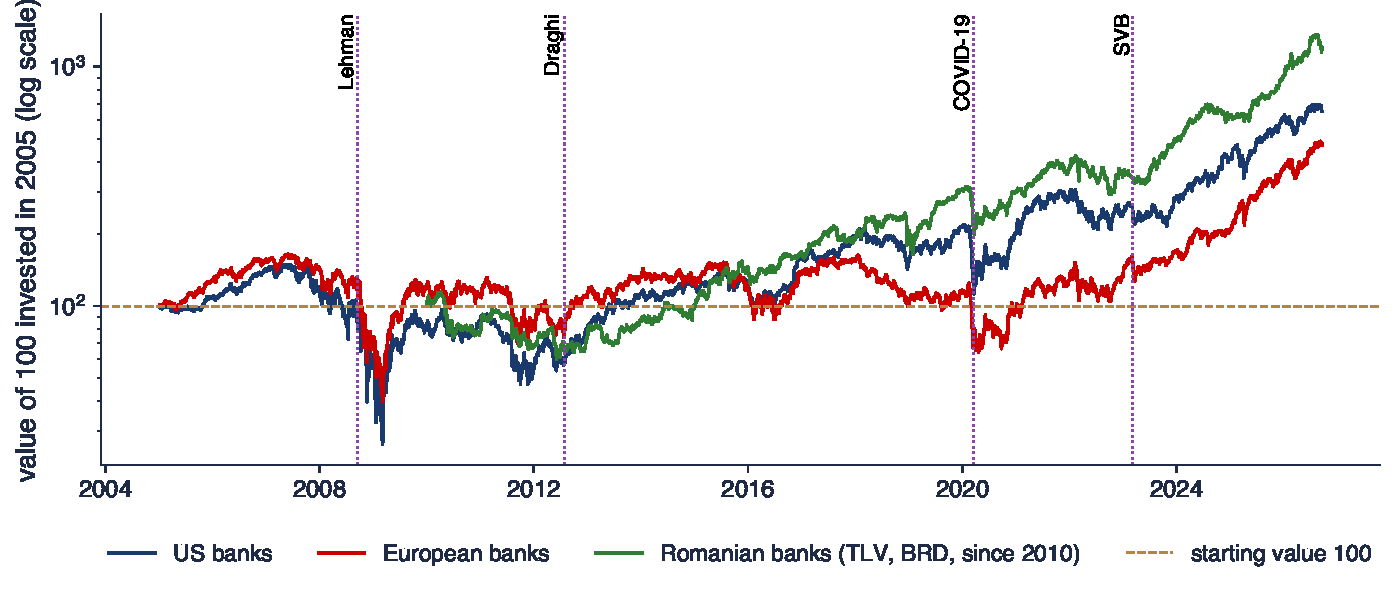
\includegraphics[width=0.97\textwidth,height=0.64\textheight,keepaspectratio]{sfm_ch15_bank_indices.pdf}
\end{center}
\vspace{-0.25cm}
\begin{itemize}
    \item Value of 100 invested in each equal-weighted portfolio (log scale); dotted lines: Lehman, Draghi's speech, COVID-19, the failure of SVB
    \item Maximum drawdown: US banks $-82\%$ (6 March 2009), European banks $-76\%$ (9 March 2009), Romanian banks $-47\%$ (5 June 2012)
\end{itemize}
\sfmquantlet{Ch_15}{SFM_ch15_crises}
\end{frame}

\begin{frame}{Interpretation of the Bank Portfolios}
\itemsize{\small}
\begin{itemize}
    \item 2008--2009: US and European banks lost about four fifths of their value; the trough came in March 2009, six months after Lehman
    \begin{itemize}
        \item a systemic crisis is a process that lasts months, not a single bad day
    \end{itemize}
    \item European banks stayed below their 2005 level for most of the period: the euro-area crisis and low interest rates
    \item Romanian banks: their worst fall came in the euro-area crisis of 2011--2012 (the parent banks of many Romanian banks are in the euro area)
    \item March 2020 and March 2023: sharp falls, but short; central banks and governments reacted within days
\end{itemize}
\end{frame}

\begin{frame}{2008: Lehman Brothers}
\itemsize{\footnotesize}
\begin{columns}[T]
\begin{column}{0.58\textwidth}
\begin{itemize}
    \item 15 September 2008: Lehman Brothers files for bankruptcy, the largest bankruptcy in US history (assets above 600 billion USD)
    \begin{itemize}
        \item 16 September: AIG, an insurer that had sold protection on mortgage debt to many banks, is rescued by the Federal Reserve
        \item the same day, a money market fund holding Lehman debt ``breaks the buck'' and investors run from such funds
    \end{itemize}
    \item All three channels at once
    \begin{itemize}
        \item direct exposures (derivatives with Lehman), common exposures (mortgages), a run on short-term funding
    \end{itemize}
    \item From the end of August to the trough in November: US banks $-59\%$, European banks $-54\%$, S\&P 500 $-41\%$
\end{itemize}
\end{column}
\begin{column}{0.38\textwidth}
\centering
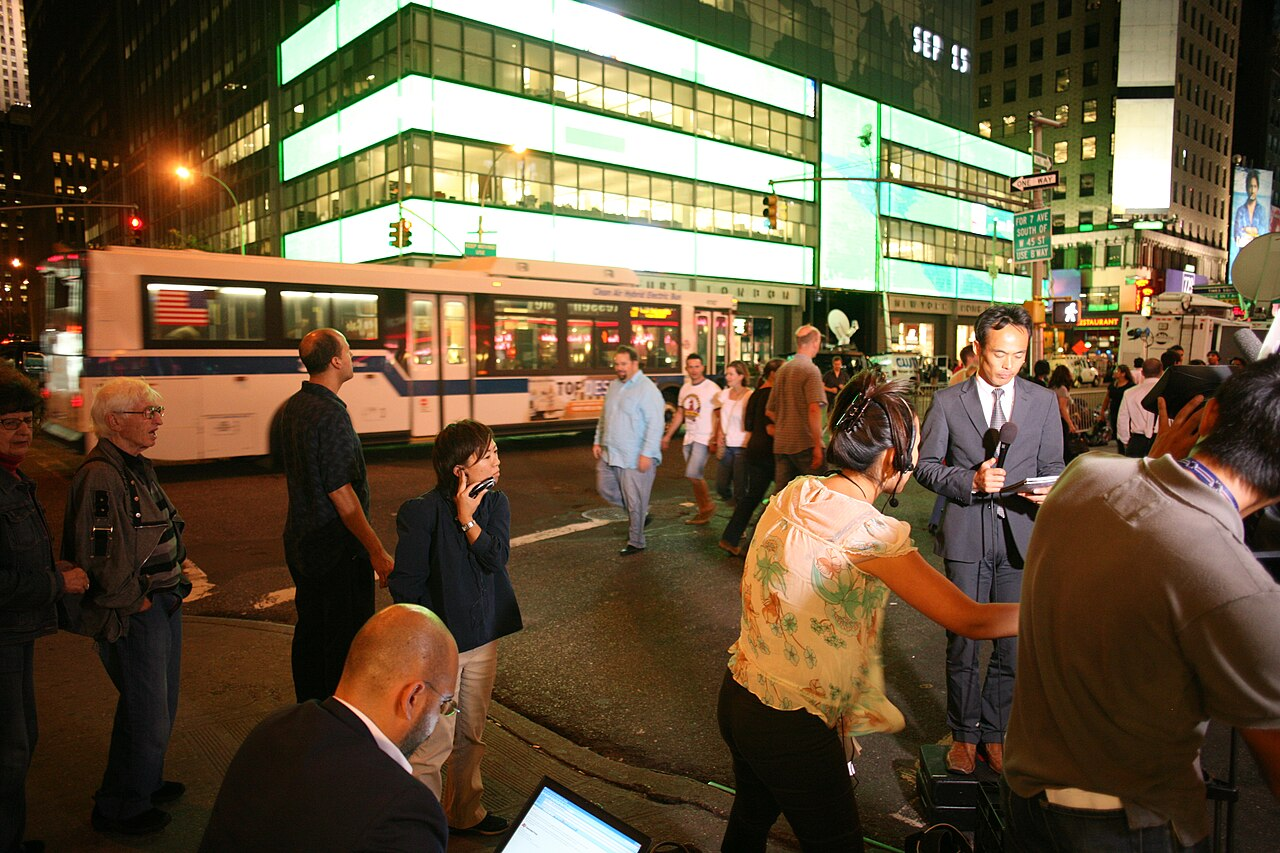
\includegraphics[height=0.40\textheight]{ch0_lehman_2008.jpg}\\[1mm]
\imgcap{Lehman Brothers headquarters, New York, 15 September 2008}
\imgcredit{https://commons.wikimedia.org/wiki/File:Lehman_Brothers-NYC-20080915.jpg}{Photo: Robert Scoble (2008); CC BY 2.0; Wikimedia Commons}
\end{column}
\end{columns}
\end{frame}

\begin{frame}{2010--2012: The Euro-Area Crisis}
\itemsize{\footnotesize}
\begin{columns}[T]
\begin{column}{0.60\textwidth}
\begin{itemize}
    \item Greece (2010), then Ireland, Portugal, Spain and Italy: doubts about government debt
    \begin{itemize}
        \item \textbf{the bank--sovereign loop}: banks hold their own government's bonds, and the government stands behind its banks
        \item a fall in bond prices weakens the banks; rescuing the banks weakens the state
    \end{itemize}
    \item 26 July 2012: Mario Draghi, President of the ECB (European Central Bank): ``the ECB is ready to do whatever it takes to preserve the euro'' \refDraghi
    \begin{itemize}
        \item a promise, not a purchase, stopped the spiral: the role of expectations
    \end{itemize}
    \item July 2011 -- September 2012, worst point: European banks $-41\%$, US banks $-37\%$, Romanian banks $-34\%$
\end{itemize}
\end{column}
\begin{column}{0.36\textwidth}
\centering

\includegraphics[height=0.30\textheight]{ch15_ecb_frankfurt_2015.jpg}\\[1mm]
\imgcap{The ECB building in Frankfurt am Main}
\imgcredit{https://commons.wikimedia.org/wiki/File:Seat_of_the_European_Central_Bank_and_Frankfurt_Skyline_at_dawn_20150422_1.jpg}{Photo: D\-XR (2015); CC BY-SA 4.0; Wikimedia Commons}
\end{column}
\end{columns}
\end{frame}

\begin{frame}{March 2020: The Dash for Cash}
\itemsize{\footnotesize}
\begin{columns}[T]
\begin{column}{0.58\textwidth}
\begin{itemize}
    \item COVID-19 lockdowns: everyone wanted cash at the same time, even government bonds were sold
    \begin{itemize}
        \item the stress started outside the banks: funds, firms, the bond market
        \item banks were better capitalised than in 2008 (Basel III) and became part of the solution (credit lines)
    \end{itemize}
    \item Fast policy response: central banks bought assets and lent in dollars to other central banks
    \begin{itemize}
        \item trough on 23 March 2020: US banks $-48\%$, European banks $-48\%$, Romanian banks $-35\%$, S\&P 500 $-34\%$
    \end{itemize}
\end{itemize}
\end{column}
\begin{column}{0.38\textwidth}
\centering
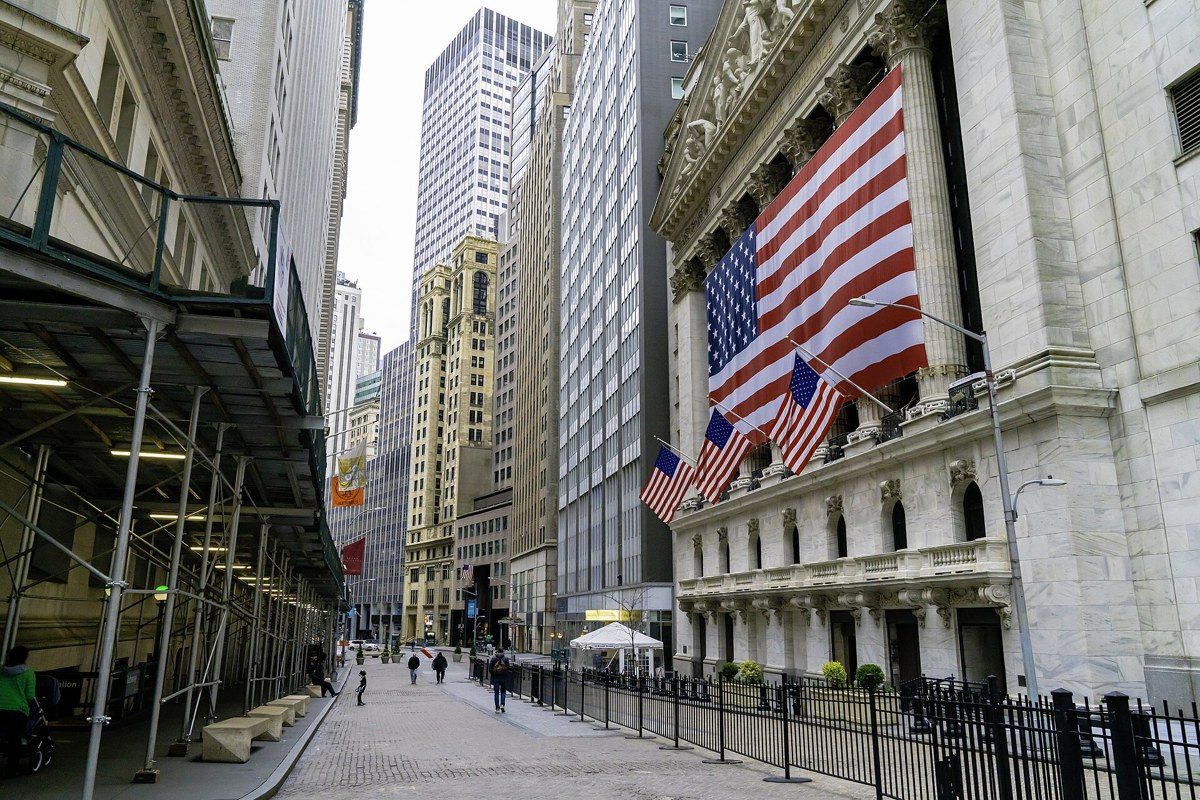
\includegraphics[height=0.38\textheight]{ch0_fidi_march_2020.jpg}\\[1mm]
\imgcap{The Financial District of New York, 25 March 2020}
\imgcredit{https://commons.wikimedia.org/wiki/File:Subdued_FiDi_(50063555551).jpg}{Photo: Billie Grace Ward (2020); CC BY 2.0; Wikimedia Commons}
\end{column}
\end{columns}
\end{frame}

\begin{frame}{March 2023: SVB}
\itemsize{\footnotesize}
\begin{columns}[T]
\begin{column}{0.58\textwidth}
\begin{itemize}
    \item SVB (Silicon Valley Bank): deposits of technology firms, mostly above the insured limit, invested in long-term bonds
    \begin{itemize}
        \item rising interest rates in 2022 created large unrealised losses on the bonds
        \item 9 March 2023: depositors tried to withdraw about 42 billion USD in one day; 10 March: the bank is closed \refFed; \refFDIC
    \end{itemize}
    \item A run in the age of mobile banking: faster than any run before
    \begin{itemize}
        \item a mid-sized bank became systemic through information contagion: other regional banks fell the next days
    \end{itemize}
\end{itemize}
\end{column}
\begin{column}{0.38\textwidth}
\centering

\includegraphics[height=0.38\textheight]{ch15_svb_hq_2023.jpg}\\[1mm]
\imgcap{Silicon Valley Bank headquarters, Santa Clara, 13 March 2023}
\imgcredit{https://commons.wikimedia.org/wiki/File:3003_West_Tasman_Drive_entrance_2,_Santa_Clara,_California.jpg}{Photo: Minh Nguyen (2023); CC BY-SA 4.0; Wikimedia Commons}
\end{column}
\end{columns}
\end{frame}

\begin{frame}{March 2023: Credit Suisse}
\itemsize{\footnotesize}
\begin{columns}[T]
\begin{column}{0.60\textwidth}
\begin{itemize}
    \item Credit Suisse: a G-SIB that had lost clients and money for years (scandals, losses on hedge-fund clients)
    \begin{itemize}
        \item after SVB, investors and depositors left quickly
    \end{itemize}
    \item 19 March 2023: takeover by UBS, approved by the Swiss supervisor FINMA \refFINMA
    \begin{itemize}
        \item AT1 bonds (additional tier 1 capital) of about 16 billion CHF were written down to zero
        \item a rescue by merger, not a resolution: too big to fail was still alive
    \end{itemize}
    \item From the end of February to the trough: European banks $-21\%$, US banks $-16\%$, Romanian banks $-7\%$
\end{itemize}
\end{column}
\begin{column}{0.36\textwidth}
\centering
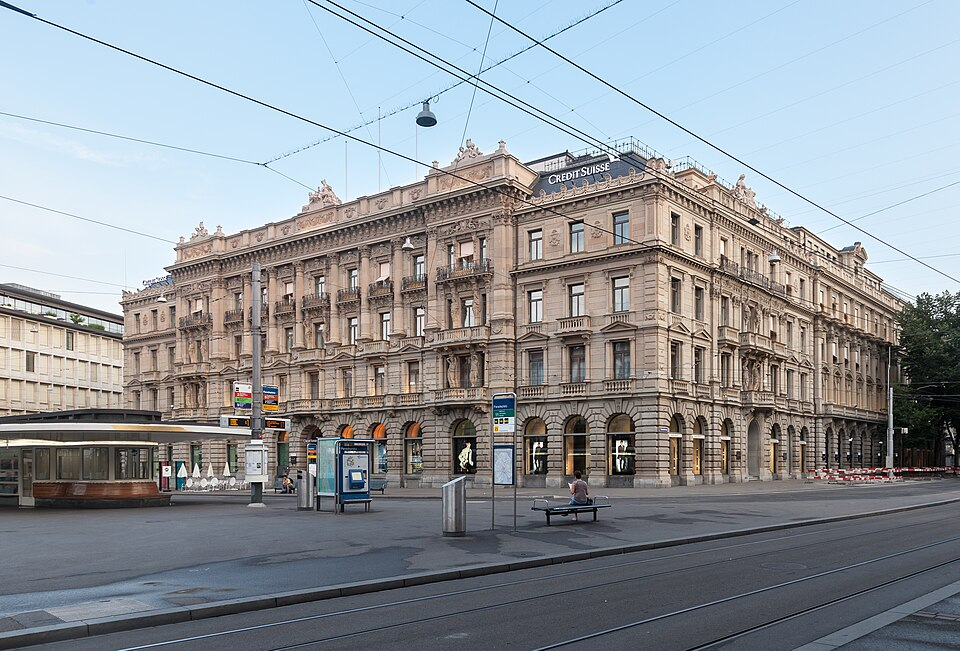
\includegraphics[height=0.28\textheight]{ch15_credit_suisse_zurich_2013.jpg}\\[1mm]
\imgcap{The Credit Suisse headquarters at Paradeplatz, Zürich}
\imgcredit{https://commons.wikimedia.org/wiki/File:Credit_Suisse_Z\%C3\%BCrich.jpg}{Photo: Thomas Wolf, www.foto-tw.de (2013); CC BY-SA 3.0 DE; Wikimedia Commons}
\end{column}
\end{columns}
\end{frame}

\begin{frame}{Four Episodes Side by Side}
\itemsize{\footnotesize}
\begin{center}
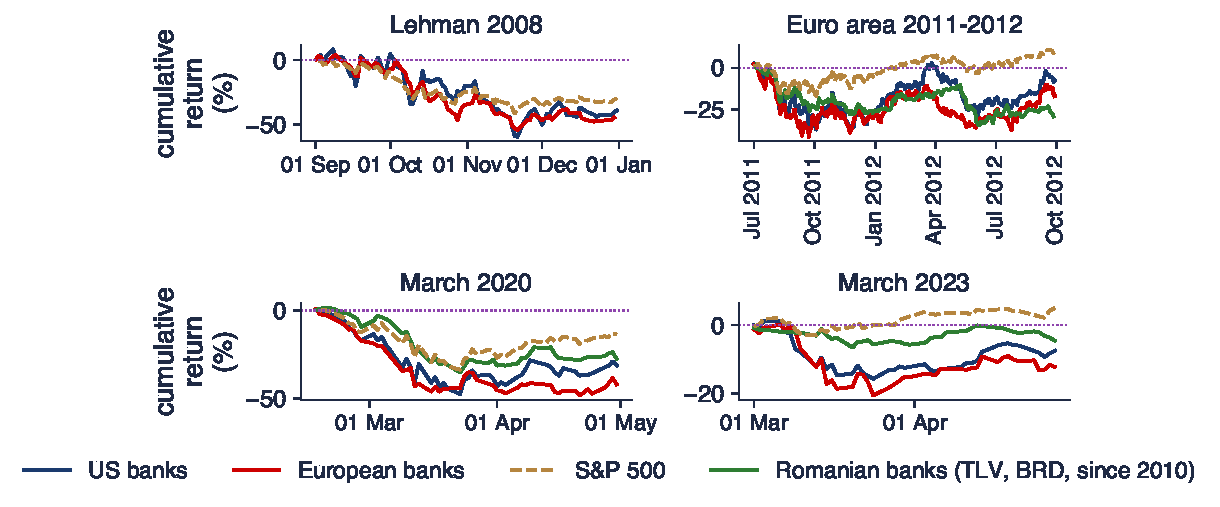
\includegraphics[width=0.97\textwidth,height=0.64\textheight,keepaspectratio]{sfm_ch15_episodes.pdf}
\end{center}
\vspace{-0.25cm}
\begin{itemize}
    \item Cumulative return from the start of each window; the Romanian banks enter the data in 2010
    \item Interpretation: in 2008 and 2011--2012 the banks fell much more than the S\&P 500 (the banks were the problem); in 2020 they fell with the market; in 2023 they fell while the market rose
\end{itemize}
\sfmquantlet{Ch_15}{SFM_ch15_crises}
\end{frame}

\begin{frame}{Recap: Four Crises}
\itemsize{\small}
\begin{itemize}
    \item 2008: contagion through derivatives, common mortgage exposures and a run on short-term funding
    \item 2011--2012: the bank--sovereign loop; stopped by a central-bank promise
    \item 2020: a shock from outside, met by better-capitalised banks; 2023: digital runs and information contagion
\end{itemize}
\end{frame}


%=============================================================================
\section{Correlation and Tail Dependence in Crises}
%=============================================================================

\begin{frame}{Correlation between Banks Rises in Crises}
\itemsize{\footnotesize}
\begin{center}
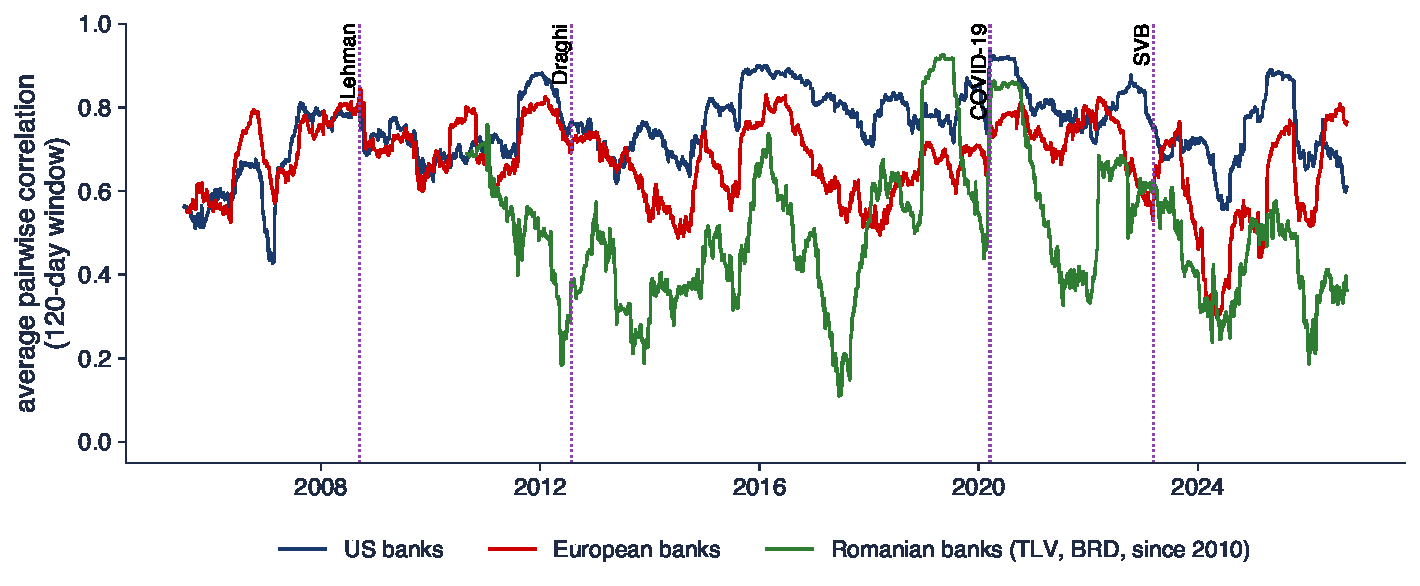
\includegraphics[width=0.97\textwidth,height=0.62\textheight,keepaspectratio]{sfm_ch15_rolling_corr.pdf}
\end{center}
\vspace{-0.25cm}
\begin{itemize}
    \item Average of the pairwise correlations of daily returns within each group, on 120-day windows
    \item US banks: $0.59$ before the crisis (July 2005 -- June 2007), up to $0.94$ (16 March 2020); TLV and BRD: $0.31$ in 2017, $0.85$ in April--June 2020
\end{itemize}
\sfmquantlet{Ch_15}{SFM_ch15_dependence}
\end{frame}

\begin{frame}{Interpretation: When Diversification Fails}
\itemsize{\small}
\begin{itemize}
    \item In crises, the banks move together: a portfolio of several banks is almost one bank
    \begin{itemize}
        \item the common factor (the market, funding stress) dominates the bank-specific news
    \end{itemize}
    \item The two Romanian banks: low correlation in calm years, very high in 2020
    \begin{itemize}
        \item in calm years the BVB stocks are driven by their own news and by low liquidity; in a crisis, by the common shock
    \end{itemize}
    \item Caution: a rolling correlation estimated on 120 days is noisy, and a rise in correlation does not prove contagion (next slide)
\end{itemize}
\end{frame}

\begin{frame}{Contagion or Interdependence? Forbes and Rigobon (1/2)}
\itemsize{\small}
\begin{itemize}
    \item If $y = \beta x + e$ with fixed $\beta$, the correlation of $x$ and $y$ rises \textbf{automatically} when the variance of $x$ rises \refFR
    \begin{itemize}
        \item $x$: the return of the source market; $y$: the return of the other market; $\beta$: the strength of the link; $e$: a shock of $y$ unrelated to $x$
        \item a higher correlation in a crisis may be the same link seen in a more volatile period: \textbf{interdependence}
        \item \textbf{contagion}: the link itself becomes stronger
    \end{itemize}
    \item Corrected correlation: \[ \rho^* = \frac{\rho}{\sqrt{1 + \delta(1 - \rho^2)}}, \qquad \delta = \frac{\sigma^2_{\text{crisis}}}{\sigma^2_{\text{calm}}} - 1 \]
    \item Notation
    \begin{itemize}
        \item $\rho$: the correlation measured in the crisis; $\sigma^2$: the variance of the source market in each period
        \item $\delta$: the relative rise of that variance; $\rho^*$: the crisis correlation that the calm-period volatility would give
        \item compare $\rho^*$ with $\rho_{\text{calm}}$: $\rho^* > \rho_{\text{calm}}$ points to contagion
    \end{itemize}
\end{itemize}
\end{frame}

\begin{frame}{Contagion or Interdependence? Forbes and Rigobon (2/2)}
\itemsize{\small}
\begin{itemize}
    \item Worked example
    \begin{itemize}
        \item US bank portfolio (source) and European bank portfolio: calm January 2005 -- June 2007 ($n = 506$), crisis 15 September -- 31 December 2008 ($n = 72$)
        \item $\rho_{\text{calm}} = 0.40$, $\rho_{\text{crisis}} = 0.60$; variance $0.89$ $\to$ $75.4$, so $\delta = 83.7$
        \item $\rho^* = 0.60/\sqrt{1 + 83.7 \times 0.64} = 0.60/\sqrt{54.4} = 0.08$
    \end{itemize}
    \item Interpretation: after the correction there is no rise in correlation: the data are consistent with interdependence, not with a stronger link
\end{itemize}
\end{frame}

\begin{frame}{Tail Dependence (\sfmchlinkt{https://danpele.github.io/SFM/EN/Courses/chapter10_var_es_backtesting.pdf}{Chapter 10}) (1/2)}
\itemsize{\small}
\begin{itemize}
    \item \textbf{Pseudo-observations}: $U = \text{rank}/(n + 1)$, the rank of a return among the $n$ returns of its series, scaled to $(0, 1)$
    \begin{itemize}
        \item $U \le 0.05$: one of the worst 5\% of days of that series; the marginal distributions no longer matter
    \end{itemize}
    \item \textbf{Lower tail dependence} at level $q$: $\lambda(q) = P(U_1 \le q \mid U_2 \le q)$
    \begin{itemize}
        \item $U_1$: the bank; $U_2$: the market; $\lambda(q)$: the probability that the bank is in its worst $q$ days, given that the market is in its worst $q$ days
        \item under independence $\lambda(q) = q$; the limit $\lambda_L = \lim_{q \to 0}\lambda(q)$ is the tail-dependence coefficient
    \end{itemize}
    \item For systemic risk: tail dependence measures how often a bank and the market are in their worst days \textbf{together}
\end{itemize}
\end{frame}

\begin{frame}{Tail Dependence (\sfmchlinkt{https://danpele.github.io/SFM/EN/Courses/chapter10_var_es_backtesting.pdf}{Chapter 10}) (2/2)}
\itemsize{\small}
\begin{itemize}
    \item The t copula (\sfmchlink{https://danpele.github.io/SFM/EN/Courses/chapter10_var_es_backtesting.pdf}{Chapter 10}) has a positive tail-dependence coefficient \refDM; the Gaussian copula has $\lambda_L = 0$ \[ \lambda_L = 2\,t_{\nu+1}\Big(-\sqrt{(\nu + 1)(1 - \rho)/(1 + \rho)}\Big) > 0 \]
    \item Notation
    \begin{itemize}
        \item $t_{\nu+1}$: the distribution function of a Student-t with $\nu + 1$ degrees of freedom
        \item $\rho$: the correlation parameter of the copula; $\nu$: its degrees of freedom; a small $\nu$ gives strong joint crashes
    \end{itemize}
    \item Estimation
    \begin{itemize}
        \item $\rho = \sin(\pi\tau/2)$ from Kendall's $\tau$, a rank correlation; $\nu$ by maximum likelihood
        \item $\tau = (C - D)/\binom{n}{2}$; $C$, $D$: the numbers of concordant and discordant pairs of days (both series move in the same or in opposite directions)
    \end{itemize}
\end{itemize}
\end{frame}

\begin{frame}{Tail Dependence of Banks and Markets}
\itemsize{\footnotesize}
\begin{center}
\scriptsize
\begin{tabular}{lrrrrrr}
\toprule
\textbf{Pair} & $n$ & corr. & $\lambda(5\%)$ & $\lambda(1\%)$ & $\hat\nu$ & $\lambda_L$ (t) \\
\midrule
US banks, S\&P 500 & 5\,229 & $0.79$ & $0.64$ & $0.63$ & $3.2$ & $0.49$ \\
European banks, Euro Stoxx 50 & 5\,212 & $0.86$ & $0.72$ & $0.67$ & $3.1$ & $0.59$ \\
Romanian banks, BET & 3\,414 & $0.86$ & $0.65$ & $0.62$ & $4.3$ & $0.53$ \\
European banks, US banks & 4\,895 & $0.59$ & $0.43$ & $0.50$ & $3.0$ & $0.36$ \\
\bottomrule
\end{tabular}
\end{center}
\begin{itemize}
    \item $\lambda(q)$: empirical; $\hat\nu$ and $\lambda_L$: t copula; under independence $\lambda(5\%) = 0.05$ and $\lambda(1\%) = 0.01$
    \item Interpretation: on more than half of the market's worst days the banks are also in their worst days; the small $\hat\nu$ (about 3--4) means strong joint crashes, which a Gaussian copula misses entirely
    \item $\lambda(1\%)$ rests on a few dozen days: an imprecise estimate
\end{itemize}\sfmquantlet{Ch_15}{SFM_ch15_dependence}
\end{frame}

\begin{frame}{Joint Bad Days}
\itemsize{\footnotesize}
\begin{center}
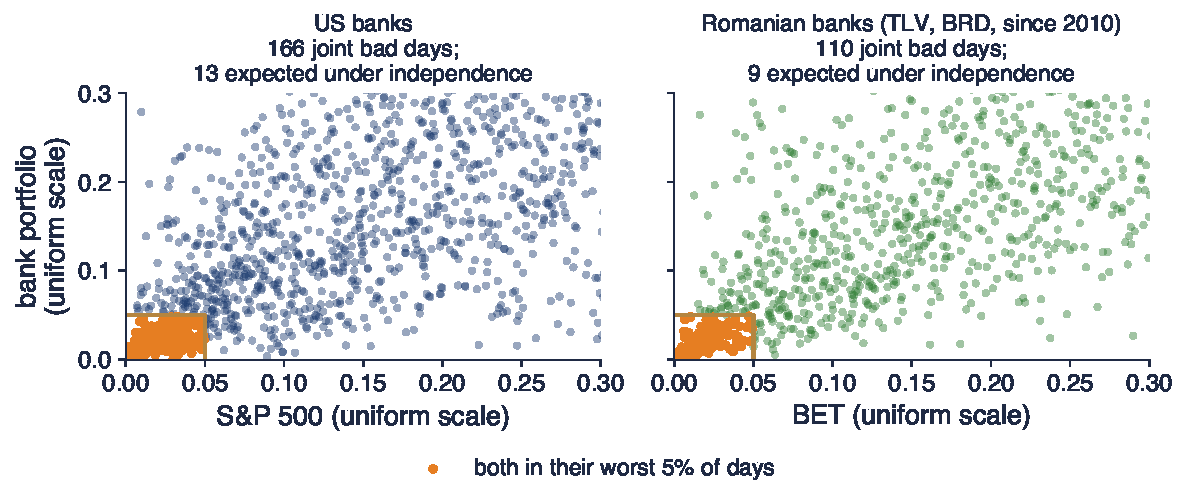
\includegraphics[width=0.97\textwidth,height=0.60\textheight,keepaspectratio]{sfm_ch15_tail_scatter.pdf}
\end{center}
\vspace{-0.25cm}
\begin{itemize}
    \item Lower-left corner of the pseudo-observations; orange: both the bank portfolio and the index in their worst 5\% of days
    \item US: 166 joint bad days against 13 under independence (about 13 times more); Romania: 110 against 9
\end{itemize}
\sfmquantlet{Ch_15}{SFM_ch15_dependence}
\end{frame}

\begin{frame}{Recap: Correlation and Tail Dependence}
\itemsize{\small}
\begin{itemize}
    \item Bank correlations rise in crises; diversification across banks fails when it is needed
    \item A rise in correlation is not proof of contagion: correct for the rise in volatility (Forbes--Rigobon)
    \item Tail dependence (t copula, $\nu$ about 3--4) shows strong joint crashes of banks and markets
\end{itemize}
\end{frame}


%=============================================================================
\section{CoVaR and Delta-CoVaR}
%=============================================================================

\begin{frame}{From VaR to CoVaR}
\itemsize{\small}
\begin{itemize}
    \item $X^i$: return of institution $i$; $X^{sys}$: return of the system; level $\alpha$ = probability of the tail (\sfmchlink{https://danpele.github.io/SFM/EN/Courses/chapter10_var_es_backtesting.pdf}{Chapter 10})
    \begin{itemize}
        \item $q_\alpha(X^i)$: the $\alpha$-quantile of $X^i$; $\mathrm{VaR}^i_\alpha = -q_\alpha(X^i)$: the loss of $i$ exceeded with probability $\alpha$
    \end{itemize}
    \item \textbf{CoVaR} (conditional VaR of the system) \refAB{} \begin{equation*} \mathrm{CoVaR}^{sys|i}_\alpha = -q_\alpha\big(X^{sys} \mid X^i = q_\alpha(X^i)\big) \end{equation*}
    \begin{itemize}
        \item $q_\alpha(X^{sys} \mid \cdot)$: the $\alpha$-quantile of the system return, conditional on what follows the bar
        \item the VaR 1\% of the system on a day when institution $i$ is at its own VaR 1\%: ``CoVaR 1\%''
    \end{itemize}
    \item $\boldsymbol{\Delta}$\textbf{CoVaR}: the contribution of $i$ to systemic risk \begin{equation*} \Delta\mathrm{CoVaR}^{sys|i}_\alpha = \mathrm{CoVaR}^{sys|X^i = q_\alpha}_\alpha - \mathrm{CoVaR}^{sys|X^i = q_{50\%}}_\alpha \end{equation*}
    \begin{itemize}
        \item $q_{50\%}$: the median of $X^i$, a normal day of the institution
        \item reading: how much the VaR of the system rises when $i$ moves from a normal day (its median) to distress
    \end{itemize}
\end{itemize}
\end{frame}

\begin{frame}{Quantile Regression (\sfmchlinkt{https://danpele.github.io/SFM/EN/Courses/chapter13_machine_learning.pdf}{Chapter 13})}
\itemsize{\small}
\begin{itemize}
    \item Linear quantile regression \refKB: $q_\alpha(Y \mid X = x) = a_\alpha + b_\alpha x$
    \begin{itemize}
        \item estimated by minimising $\sum_t \rho_\alpha(y_t - a - bx_t)$, with the check loss $\rho_\alpha(u) = u(\alpha - \mathbf{1}\{u < 0\})$
        \item $u$: the residual; $\mathbf{1}\{u < 0\}$: 1 if the point is below the line, 0 otherwise
        \item for $\alpha = 1\%$, a residual below the line costs 99 times more than one above it: the line passes below 99\% of the points
    \end{itemize}
    \item Same idea as VaR 1\% by quantile regression in \sfmchlink{https://danpele.github.io/SFM/EN/Courses/chapter13_machine_learning.pdf}{Chapter 13}, now with another institution as the regressor
    \begin{itemize}
        \item the slope $b_\alpha$ can differ from the OLS slope: the tail can react more strongly than the centre
    \end{itemize}
    \item $a_\alpha$ is the intercept (constant term) of the regression, $b_\alpha$ the slope
\end{itemize}
\end{frame}

\begin{frame}{Estimating CoVaR in Three Steps}
\itemsize{\small}
\begin{itemize}
    \item \textbf{Step 1}: quantile regression of the system on the institution at level $\alpha$: $X^{sys}_t = a + bX^i_t + \varepsilon_t$ \refAB
    \begin{itemize}
        \item $\hat a$, $\hat b$: the estimated intercept and slope; the $\alpha$-quantile of the error $\varepsilon_t$ is zero by construction
    \end{itemize}
    \item \textbf{Step 2}: the empirical quantiles of the institution: $\hat q_\alpha(X^i)$ (distress) and $\hat q_{50\%}(X^i)$ (median)
    \item \textbf{Step 3}: plug in
    \begin{itemize}
        \item $\mathrm{CoVaR}_\alpha = -(\hat a + \hat b\,\hat q_\alpha(X^i))$
        \item $\Delta\mathrm{CoVaR}_\alpha = \hat b\,\big(\hat q_{50\%}(X^i) - \hat q_\alpha(X^i)\big)$: only the slope and the distance between the two quantiles matter
    \end{itemize}
    \item Here the system is proxied by the regional equity index (S\&P 500, Euro Stoxx 50, BET); Adrian and Brunnermeier use the portfolio of all financial institutions
\end{itemize}
\end{frame}

\begin{frame}{Worked Example: JPMorgan Chase and the S\&P 500}
\itemsize{\small}
\begin{itemize}
    \item Daily log returns, 2005--2026 ($n = 5\,229$); quantile regression at 1\%: $\hat a = -2.35$, $\hat b = 0.39$
    \begin{itemize}
        \item JPM: $\hat q_{1\%} = -6.27\%$ (so VaR 1\% of JPM $= 6.27\%$), median $\hat q_{50\%} = 0.07\%$
    \end{itemize}
    \item \textbf{CoVaR 1\%} $= -(-2.35 + 0.39 \times (-6.27)) = 2.35 + 2.44 = 4.79\%$
    \begin{itemize}
        \item CoVaR at the median of JPM: $2.32\%$
    \end{itemize}
    \item \textbf{$\Delta$CoVaR 1\%} $= 0.39 \times (0.07 - (-6.27)) = 0.39 \times 6.34 = 2.47\%$
    \begin{itemize}
        \item the unconditional VaR 1\% of the S\&P 500 is $3.53\%$
    \end{itemize}
    \item Interpretation: when JPM is in distress, the loss of the index exceeded with probability 1\% is 4.79\%, against 2.32\% on a normal JPM day
\end{itemize}
\end{frame}

\begin{frame}{CoVaR in a Picture}
\itemsize{\footnotesize}
\begin{center}
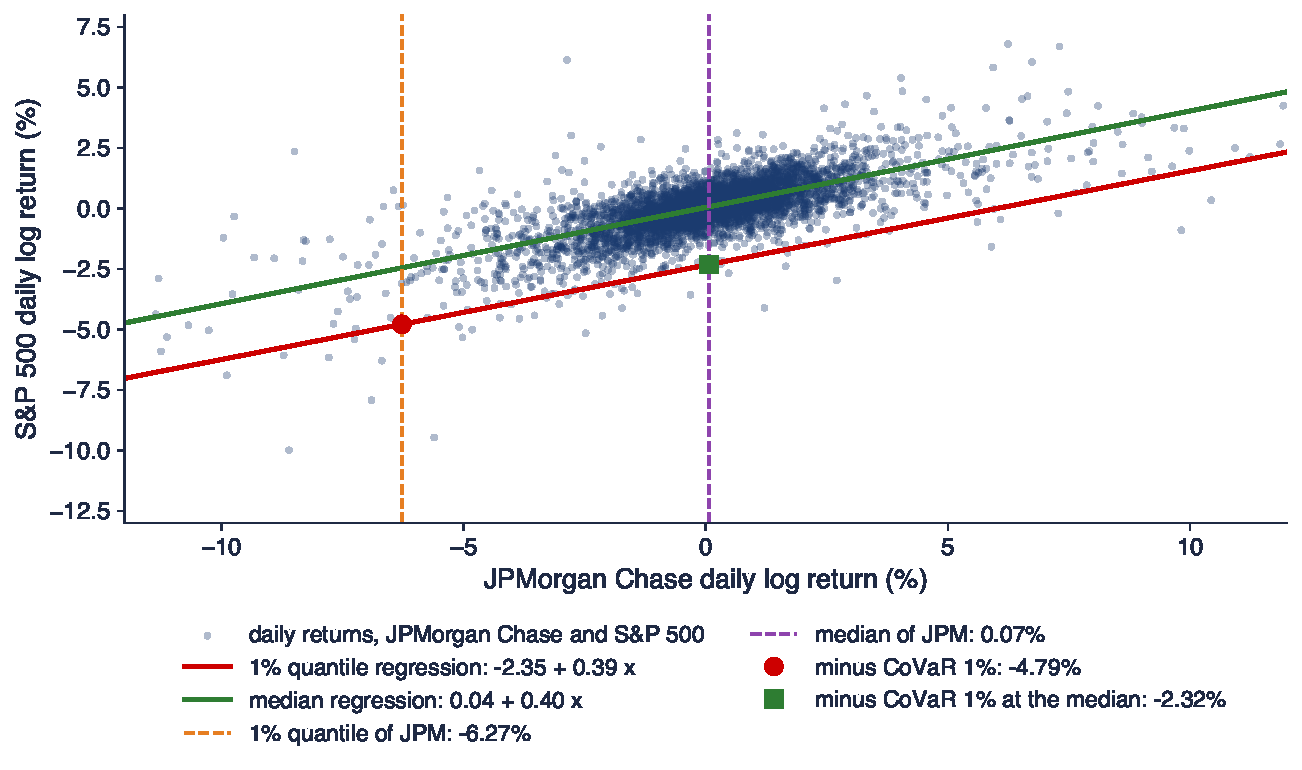
\includegraphics[width=0.97\textwidth,height=0.60\textheight,keepaspectratio]{sfm_ch15_covar_qr.pdf}
\end{center}
\vspace{-0.25cm}
\begin{itemize}
    \item Red line: the 1\% quantile of the S\&P 500 given JPM; green line: the median; dashed: the 1\% quantile and the median of JPM
    \item $\Delta$CoVaR is the vertical distance between the red dot and the green square on the red line: $2.47\%$
\end{itemize}
\sfmquantlet{Ch_15}{SFM_ch15_covar}
\end{frame}

\begin{frame}{$\Delta$CoVaR 1\% of 13 Banks}
\itemsize{\footnotesize}
\begin{center}
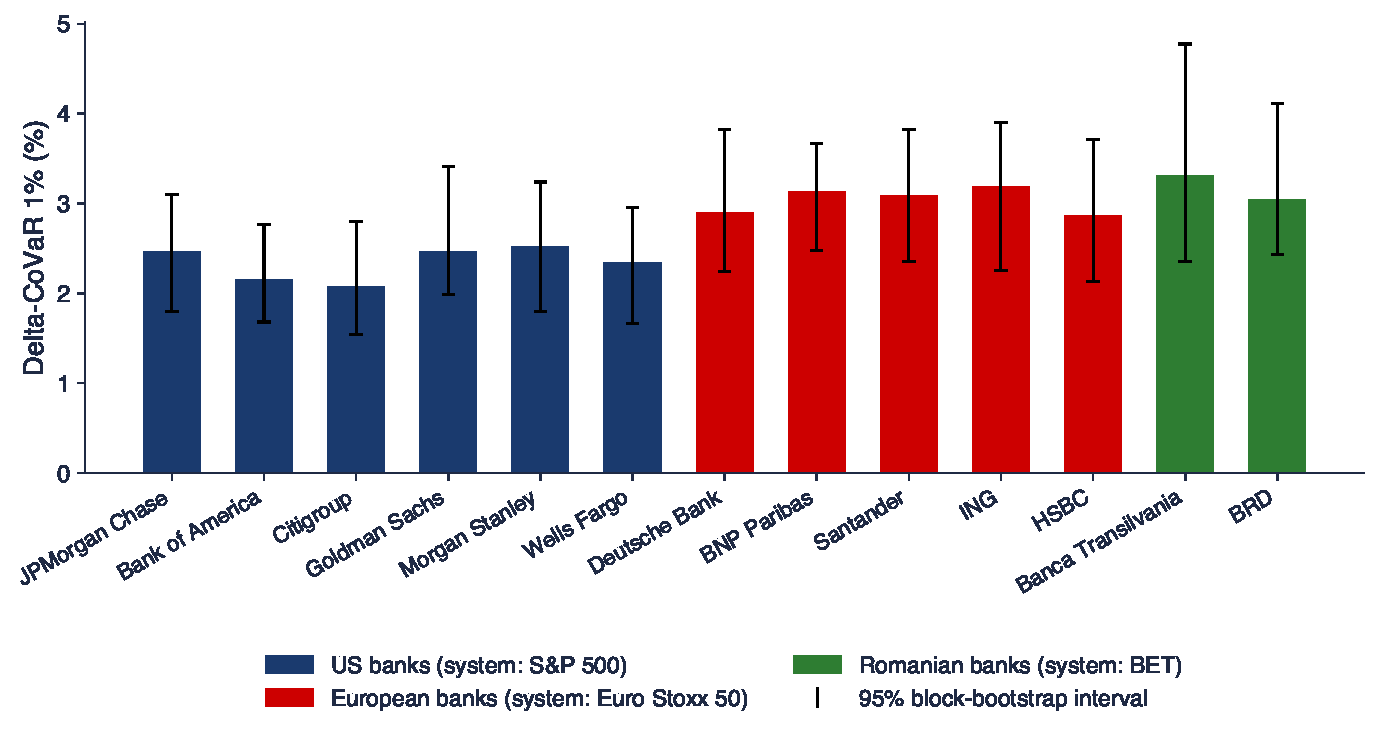
\includegraphics[width=0.97\textwidth,height=0.62\textheight,keepaspectratio]{sfm_ch15_dcovar.pdf}
\end{center}
\vspace{-0.25cm}
\begin{itemize}
    \item System: the regional index; 95\% intervals from a moving-block bootstrap (blocks of 20 days, 200 resamples)
    \item US banks: 2.1--2.5\%; European banks: 2.9--3.2\%; TLV $3.31\%$, BRD $3.05\%$; largest: Banca Transilvania
\end{itemize}
\sfmquantlet{Ch_15}{SFM_ch15_covar}
\end{frame}

\begin{frame}{Interpretation of $\Delta$CoVaR}
\itemsize{\small}
\begin{itemize}
    \item The intervals overlap: within a region, the data cannot rank the banks precisely
    \begin{itemize}
        \item a ranking of systemic importance needs its uncertainty, like any estimate (bootstrap, \sfmchlink{https://danpele.github.io/SFM/EN/Courses/chapter2_classical_distributions_stylised_facts.pdf}{Chapter 2})
    \end{itemize}
    \item European and Romanian banks have a larger $\Delta$CoVaR than US banks
    \begin{itemize}
        \item banks weigh more in the Euro Stoxx 50 and in the BET than in the S\&P 500: the index is closer to a banking system
        \item TLV and BRD are among the largest stocks of the BET, so the BET partly measures themselves
    \end{itemize}
    \item Robustness: the ranking at 5\% is close to the ranking at 1\% (Spearman correlation $0.87$)
    \begin{itemize}
        \item Spearman: the correlation of the ranks, $\rho_S = 1 - 6\sum_i d_i^2/(N(N^2 - 1))$; $d_i$: the difference of the two ranks of bank $i$; $N$: the number of banks
    \end{itemize}
\end{itemize}
\end{frame}

\begin{frame}{Worked Example: Banca Transilvania and the BET}
\itemsize{\small}
\begin{itemize}
    \item TLV and the BET, daily log returns since 2010 ($n = 3\,414$); quantile regression at 1\%: $\hat b = 0.61$
    \begin{itemize}
        \item TLV: $\hat q_{1\%} = -5.23\%$ (VaR 1\% of TLV), median $0.18\%$
    \end{itemize}
    \item $\Delta$CoVaR 1\% $= 0.61 \times (0.18 + 5.23) = 3.31\%$; CoVaR 1\% of the BET $= 5.28\%$
    \begin{itemize}
        \item 95\% block-bootstrap interval for $\Delta$CoVaR: [2.35, 4.78]
    \end{itemize}
    \item Interpretation: a distress day of TLV moves the 1\% quantile of the BET down by about 3.31 percentage points
    \begin{itemize}
        \item part of this is mechanical: TLV is one of the largest weights in the BET; a cleaner system would be the BET without TLV
    \end{itemize}
\end{itemize}
\end{frame}

\begin{frame}{VaR Is Not $\Delta$CoVaR}
\itemsize{\footnotesize}
\begin{center}
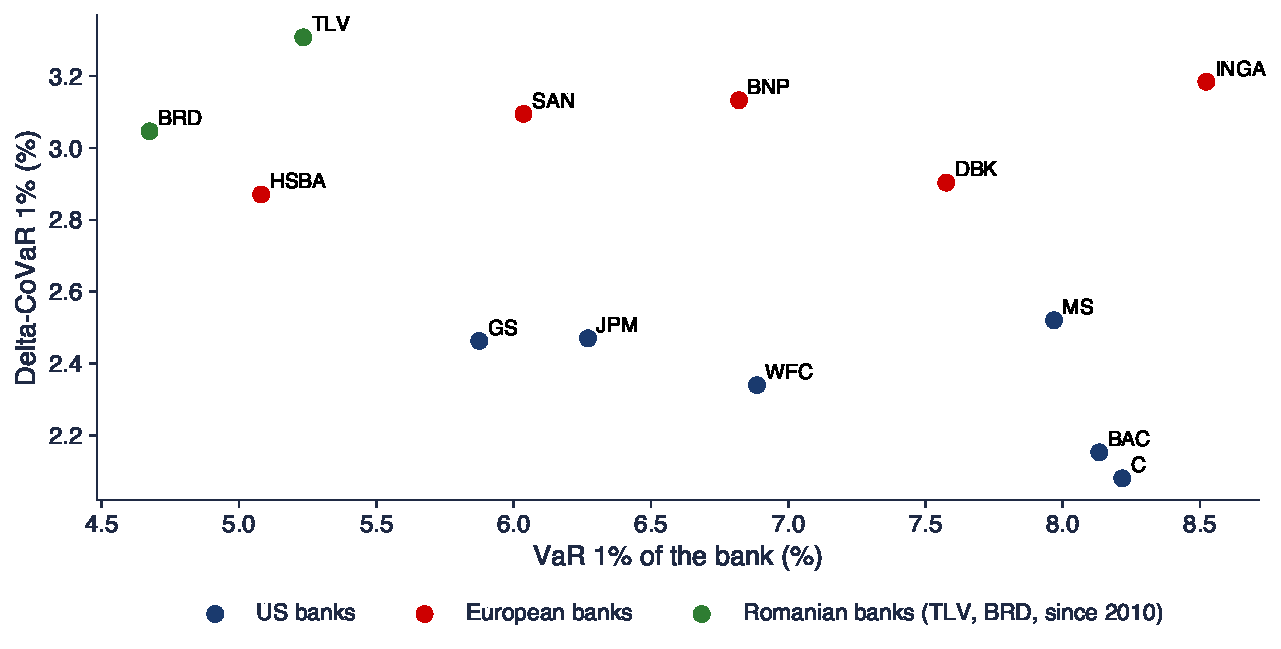
\includegraphics[width=0.97\textwidth,height=0.60\textheight,keepaspectratio]{sfm_ch15_var_vs_dcovar.pdf}
\end{center}
\vspace{-0.25cm}
\begin{itemize}
    \item Each point: a bank, its own VaR 1\% (horizontal) and its $\Delta$CoVaR 1\% (vertical); Spearman rank correlation $-0.31$
    \item Interpretation: Citigroup and Bank of America are among the three largest VaR 1\% and among the three smallest $\Delta$CoVaR; regulating banks by their own VaR misses systemic risk \refAB
\end{itemize}
\sfmquantlet{Ch_15}{SFM_ch15_covar}
\end{frame}

\begin{frame}{Time-Varying $\Delta$CoVaR}
\itemsize{\small}
\begin{itemize}
    \item Adrian and Brunnermeier let the quantiles depend on lagged \textbf{state variables} $M_{t-1}$ \refAB
    \begin{itemize}
        \item $M_{t-1}$: the vector of state variables known at the close of day $t - 1$ (market stress, interest rates)
        \item $X^i_t = c + \gamma^\top M_{t-1}$ at levels $\alpha$ and 50\%: $\hat q_{\alpha,t}(X^i)$ and $\hat q_{50\%,t}(X^i)$
        \item $X^{sys}_t = a + bX^i_t + \delta^\top M_{t-1}$ at level $\alpha$; then $\Delta\mathrm{CoVaR}_t = \hat b\,(\hat q_{50\%,t} - \hat q_{\alpha,t})$
        \item $c$, $\gamma$, $a$, $b$, $\delta$: coefficients of the quantile regressions ($\delta$ is not the $\delta$ of Forbes--Rigobon)
    \end{itemize}
    \item The paper uses seven state variables (VIX, liquidity and credit spreads, interest rates, market and real-estate returns)
    \begin{itemize}
        \item here, a reduced set: the VIX level and the index return of the previous day
    \end{itemize}
    \item The slope $\hat b$ is fixed; the time variation comes from the distance between the two conditional quantiles of the bank
\end{itemize}
\end{frame}

\begin{frame}{$\Delta$CoVaR 1\% through Time}
\itemsize{\footnotesize}
\begin{center}
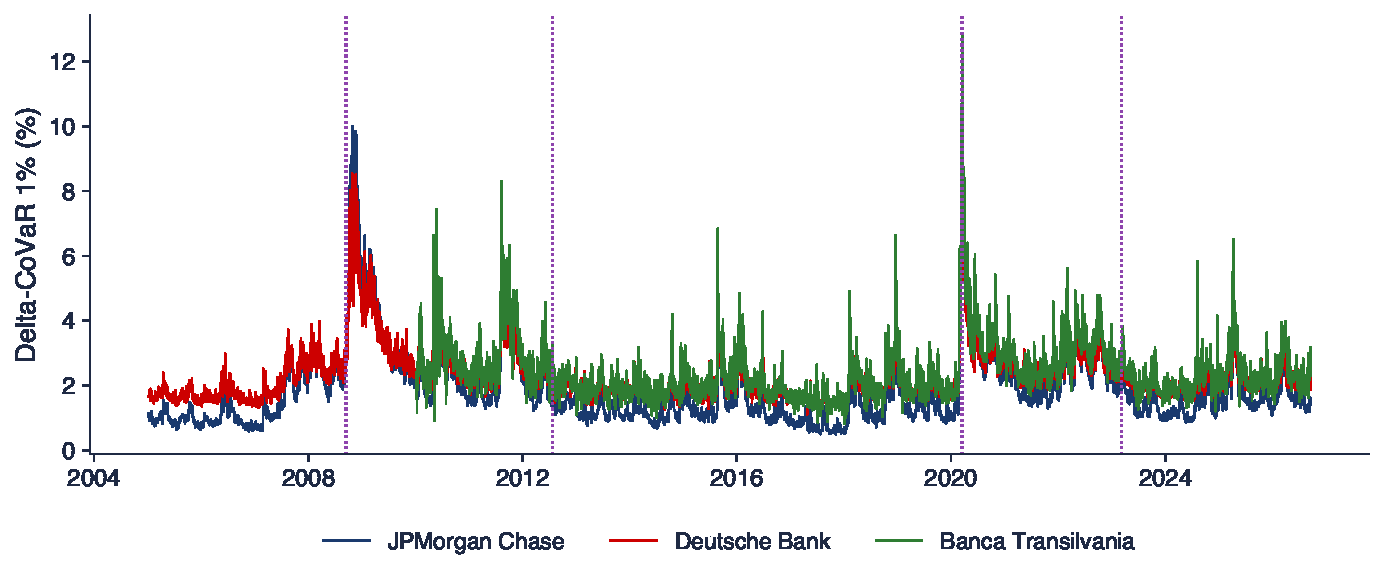
\includegraphics[width=0.97\textwidth,height=0.60\textheight,keepaspectratio]{sfm_ch15_dcovar_dynamic.pdf}
\end{center}
\vspace{-0.25cm}
\begin{itemize}
    \item JPMorgan Chase: average $1.86\%$, maximum $10.07\%$ (18 March 2020); Deutsche Bank: maximum $9.08\%$ (13 March 2020); Banca Transilvania: maximum $12.81\%$ (17 March 2020)
    \item Interpretation: the contribution of a bank to systemic risk is not a constant; it jumps when the VIX jumps (2008, March 2020) and is small in calm years (JPM in 2017: $0.75\%$)
\end{itemize}
\sfmquantlet{Ch_15}{SFM_ch15_covar}
\end{frame}

\begin{frame}{Case Study: Adrian and Brunnermeier (2016)}
\itemsize{\footnotesize}
\begin{columns}[T]
\begin{column}{0.56\textwidth}
\begin{itemize}
    \item \refAB: CoVaR of US financial institutions (commercial and investment banks, insurers, brokers), weekly data 1986--2010
    \begin{itemize}
        \item the system: the portfolio of all financial institutions; seven state variables
    \end{itemize}
    \item Findings
    \begin{itemize}
        \item in the cross-section, the VaR of an institution says little about its $\Delta$CoVaR
        \item \textbf{forward} $\Delta$CoVaR: size, leverage and maturity mismatch two years earlier predict the contribution in a crisis
        \item a basis for countercyclical capital: charge banks when risk is built up, not when it shows
    \end{itemize}
\end{itemize}
\end{column}
\begin{column}{0.42\textwidth}
\begin{columns}[T]
\begin{column}{0.48\textwidth}
\centering

\includegraphics[height=0.32\textheight]{ch15_adrian_2025.jpg}\\[1mm]
\imgcap{Tobias Adrian}
\imgcredit{https://commons.wikimedia.org/wiki/File:Tobias_Adrian_2025.jpg}{Photo: Chianoo Adrian (2025); CC BY 4.0; Wikimedia Commons}
\end{column}
\begin{column}{0.48\textwidth}
\centering

\includegraphics[height=0.32\textheight]{ch15_brunnermeier_2015.jpg}\\[1mm]
\imgcap{Markus Brunnermeier}
\imgcredit{https://commons.wikimedia.org/wiki/File:Markus_Konrad_Brunnermeier.jpg}{Photo: Iitkgpswapnil (2015); CC BY-SA 4.0; Wikimedia Commons}
\end{column}
\end{columns}
\end{column}
\end{columns}
\end{frame}

\begin{frame}{Recap: CoVaR}
\itemsize{\small}
\begin{itemize}
    \item CoVaR 1\%: the VaR 1\% of the system when the institution is at its own VaR 1\%; $\Delta$CoVaR: the rise from a normal day to distress
    \item Estimated by quantile regression: $\Delta$CoVaR $= \hat b\,(\hat q_{50\%} - \hat q_\alpha)$
    \item A bank's own VaR and its systemic contribution rank banks differently; $\Delta$CoVaR varies strongly in time
\end{itemize}
\end{frame}


%=============================================================================
\section{MES and SRISK}
%=============================================================================

\begin{frame}{Marginal Expected Shortfall}
\itemsize{\small}
\begin{itemize}
    \item \textbf{MES} \refAPPR: the expected loss of institution $i$ on the days when the market is in its tail
    \begin{itemize}
        \item $\mathrm{MES}^i_\alpha = -E\big[X^i \mid X^m \le q_\alpha(X^m)\big]$; we use the worst 5\% of market days: ``MES 5\%''
        \item $X^m$: the market return; $q_\alpha(X^m)$: its $\alpha$-quantile; the bar: ``on the days when''
        \item the direction is the opposite of CoVaR: the bank given the market, not the market given the bank
    \end{itemize}
    \item Why ``marginal'': ES of the market $= \sum_i w_i\,\mathrm{MES}^i$ when the market is a portfolio with weights $w_i$
    \begin{itemize}
        \item MES is the contribution of $i$ to the ES of the system (\sfmchlink{https://danpele.github.io/SFM/EN/Courses/chapter10_var_es_backtesting.pdf}{Chapter 10})
    \end{itemize}
    \item Estimation: sort the days by the market return, take the worst $\lceil n\alpha \rceil$ days, average the bank's returns on those days, change the sign
\end{itemize}
\end{frame}

\begin{frame}{Worked Example: MES from Ten Days}
\itemsize{\small}
\begin{center}
\footnotesize
\begin{tabular}{lrrrrrrrrrr}
\toprule
Day & 1 & 2 & 3 & 4 & 5 & 6 & 7 & 8 & 9 & 10 \\
\midrule
market & $-4.0$ & $1.2$ & $-0.5$ & $2.1$ & $-6.0$ & $0.3$ & $-1.1$ & $0.8$ & $-2.2$ & $1.5$ \\
bank & $-6.5$ & $1.8$ & $-0.2$ & $2.9$ & $-9.0$ & $0.1$ & $-2.0$ & $1.1$ & $-3.1$ & $2.4$ \\
\bottomrule
\end{tabular}
\end{center}
\begin{itemize}
    \item Level $\alpha = 20\%$: $\lceil 10 \times 0.2 \rceil = 2$ worst market days: day 5 ($-6.0$) and day 1 ($-4.0$)
    \begin{itemize}
        \item MES 20\% $= -(-9.0 - 6.5)/2 = 7.75\%$; ES 20\% of the market $= -(-6.0 - 4.0)/2 = 5.00\%$
    \end{itemize}
    \item Interpretation: on the market's bad days this bank loses about 1.5 times as much as the market: it amplifies the crashes
    \item Note: MES selects the days by the market return, not by the bank return
\end{itemize}
\end{frame}

\begin{frame}{MES 5\% of 13 Banks}
\itemsize{\footnotesize}
\begin{center}
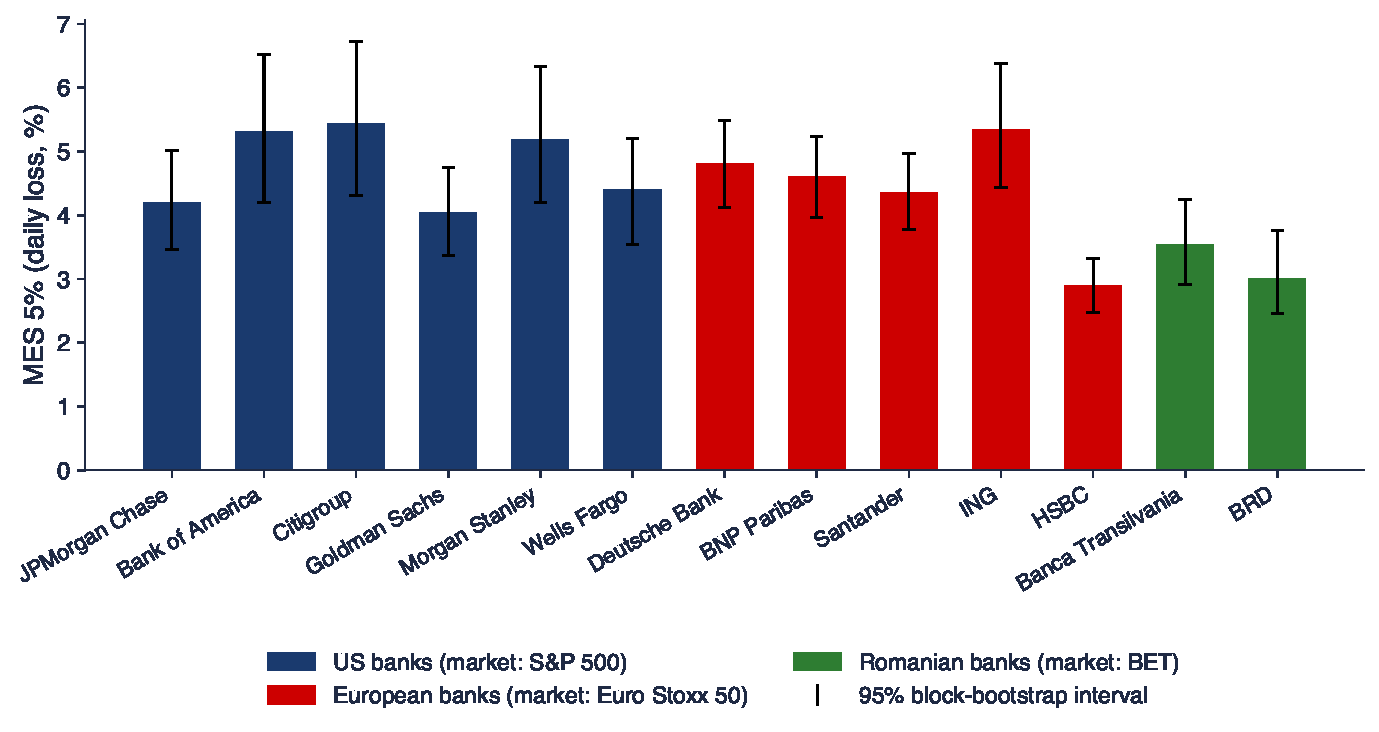
\includegraphics[width=0.97\textwidth,height=0.60\textheight,keepaspectratio]{sfm_ch15_mes.pdf}
\end{center}
\vspace{-0.25cm}
\begin{itemize}
    \item Average daily loss of each bank on the worst 5\% of days of its regional index (US and Europe since 2005, Romania since 2010); 95\% block-bootstrap intervals
    \item Largest: Citigroup ($5.44\%$) and ING ($5.35\%$); smallest: HSBC ($2.90\%$); TLV $3.54\%$, BRD $3.00\%$
\end{itemize}
\sfmquantlet{Ch_15}{SFM_ch15_mes_srisk}
\end{frame}

\begin{frame}{Interpretation: MES and $\Delta$CoVaR}
\itemsize{\small}
\begin{itemize}
    \item MES is close to a tail beta: the average market loss on its worst 5\% of days times the sensitivity of the bank
    \begin{itemize}
        \item Citigroup: OLS beta $1.66$, MES $5.44\%$; HSBC: beta $0.81$, MES $2.90\%$
    \end{itemize}
    \item MES and $\Delta$CoVaR rank the 13 banks differently: Spearman correlation $-0.29$
    \begin{itemize}
        \item they answer different questions: ``who suffers in a crash'' against ``who adds to the crash''
        \item a regulator should look at several measures, with their intervals \refBCHP
    \end{itemize}
\end{itemize}
\end{frame}

\begin{frame}{Case Study: Did MES Predict the 2008 Losses?}
\itemsize{\footnotesize}
\begin{center}
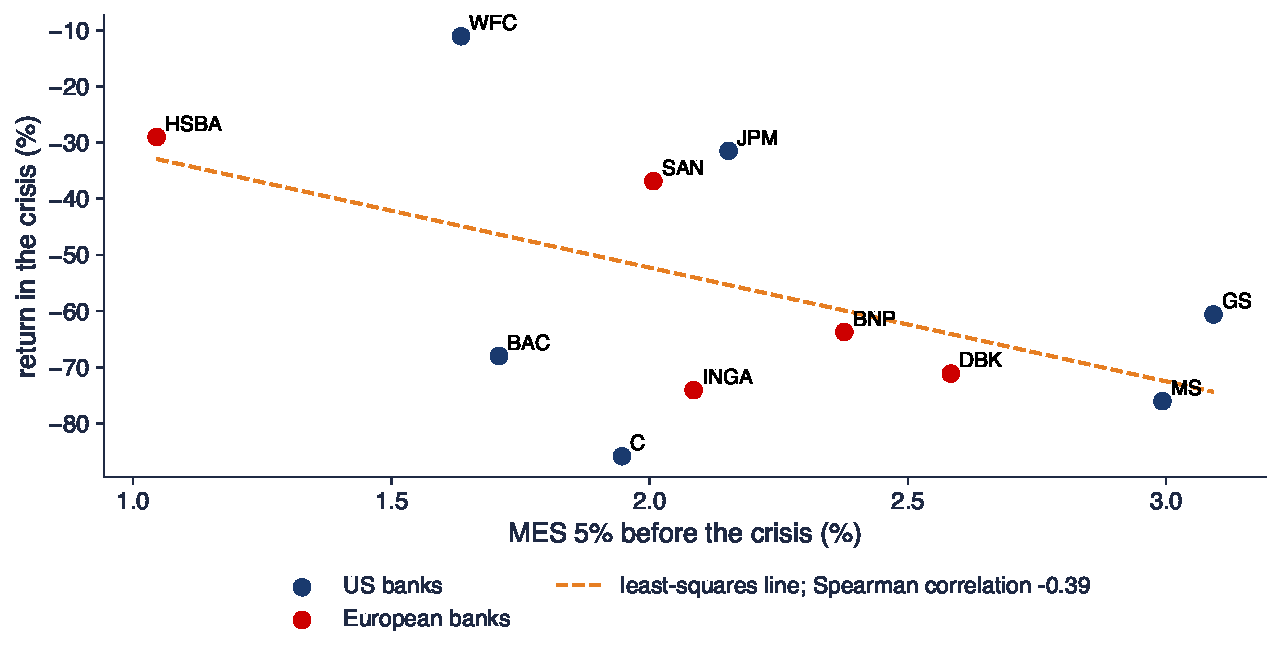
\includegraphics[width=0.97\textwidth,height=0.58\textheight,keepaspectratio]{sfm_ch15_mes_crisis.pdf}
\end{center}
\vspace{-0.25cm}
\begin{itemize}
    \item Design of \refAPPR: MES 5\% measured from June 2006 to June 2007, against the return from July 2007 to December 2008; here 11 US and European banks
    \item Spearman correlation $-0.39$ (p $= 0.23$, $n = 11$): the sign of the paper (higher MES, larger loss), but not significant with 11 banks; worst return: Citigroup ($-86\%$)
\end{itemize}
\sfmquantlet{Ch_15}{SFM_ch15_mes_srisk}
\end{frame}

\begin{frame}{From MES to LRMES}
\itemsize{\small}
\begin{itemize}
    \item A crisis lasts months: we need the loss of the bank if the market falls 40\% over six months: \textbf{LRMES} (long-run MES)
    \begin{itemize}
        \item approximation of \refAER: $\mathrm{LRMES} \approx 1 - \exp(-18 \times \mathrm{MES})$, with MES the daily loss (as a fraction) on the days when the market falls by more than 2\%
        \item the factor 18 turns the daily loss on bad days into the loss over a six-month crisis; $1 - e^{-x}$ keeps LRMES between 0 and 1
    \end{itemize}
    \item Example: MES $= 3\% = 0.03$: $\mathrm{LRMES} = 1 - e^{-0.54} = 1 - 0.583 = 41.7\%$
    \begin{itemize}
        \item the bank would lose about 41.7\% of its market value in such a crisis
    \end{itemize}
    \item Our 13 banks: LRMES between 40\% and 65\%; Brownlees and Engle estimate it instead from a dynamic model (GARCH and dynamic correlation) \refBE
\end{itemize}
\end{frame}

\begin{frame}{SRISK: the Capital Shortfall in a Crisis}
\itemsize{\small}
\begin{itemize}
    \item A bank needs equity of at least a fraction $k$ of its assets; $k = 8\%$ in \refBE
    \begin{itemize}
        \item $D$: book value of debt; $W$: market value of equity; assets $\approx D + W$
    \end{itemize}
    \item \textbf{SRISK} $= k(D + W_{\text{crisis}}) - W_{\text{crisis}}$ with $W_{\text{crisis}} = (1 - \mathrm{LRMES})W$:
    \begin{itemize}
        \item $\mathrm{SRISK} = kD - (1 - k)(1 - \mathrm{LRMES})\,W$ \refBE
        \item $kD$: the capital required on the debt; $(1 - k)(1 - \mathrm{LRMES})W$: the equity left after the crisis, net of the capital required on it
        \item SRISK $> 0$: capital missing in a crisis; the \textbf{aggregate SRISK} (sum of the positive values) is what the state might have to cover
    \end{itemize}
    \item Example: $D = 900$, $W = 100$ (billion), LRMES $= 41.7\%$
    \begin{itemize}
        \item SRISK $= 0.08 \times 900 - 0.92 \times (1 - 41.7\%) \times 100 = 72 - 53.6 = 18.4$ billion
    \end{itemize}
\end{itemize}
\end{frame}

\begin{frame}{SRISK and Leverage}
\itemsize{\footnotesize}
\begin{center}
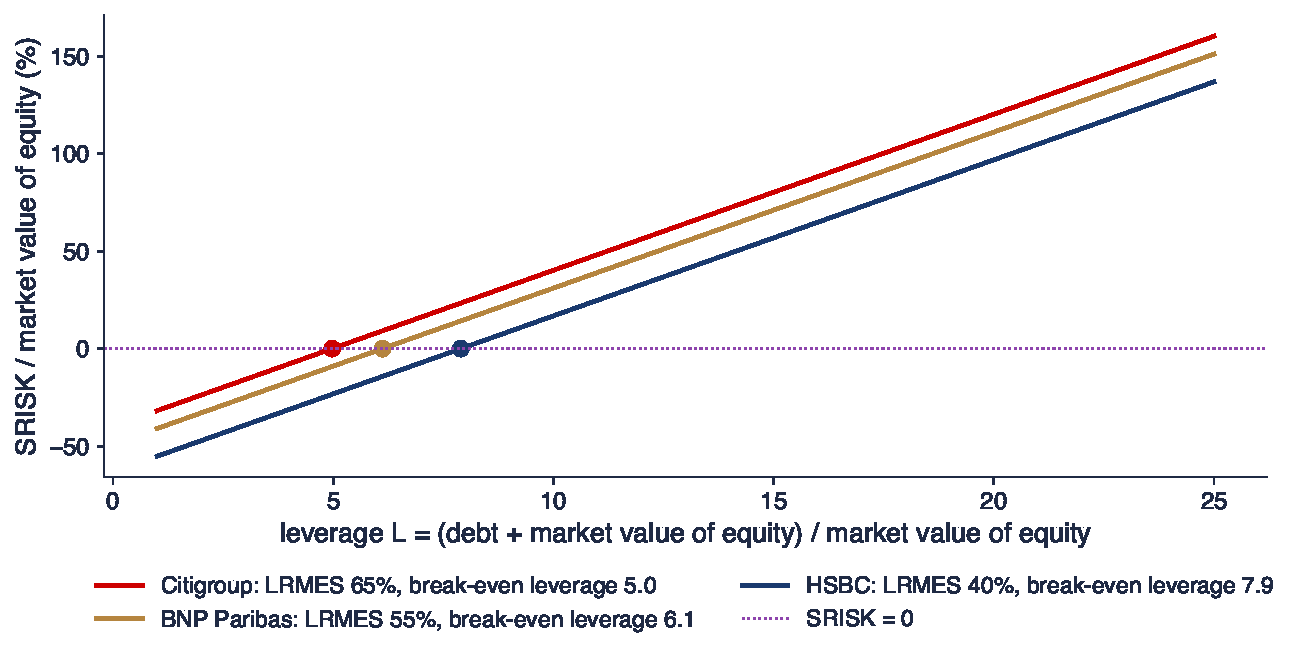
\includegraphics[width=0.97\textwidth,height=0.58\textheight,keepaspectratio]{sfm_ch15_srisk.pdf}
\end{center}
\vspace{-0.25cm}
\begin{itemize}
    \item SRISK$/W = k(L - 1) - (1 - k)(1 - \mathrm{LRMES})$ with leverage $L = (D + W)/W$; SRISK $> 0$ above $L^* = 1 + (1 - k)(1 - \mathrm{LRMES})/k$
    \item Interpretation: Citigroup needs capital in a crisis above a leverage of 5.0, HSBC only above 7.9; banks typically have $L$ between 10 and 20, so leverage decides the sign
\end{itemize}
\sfmquantlet{Ch_15}{SFM_ch15_mes_srisk}
\end{frame}

\begin{frame}{Case Study: SRISK and V-Lab}
\itemsize{\footnotesize}
\begin{columns}[T]
\begin{column}{0.56\textwidth}
\begin{itemize}
    \item \refBE: SRISK of large US financial firms, with LRMES from a GARCH--DCC model (\sfmchlink{https://danpele.github.io/SFM/EN/Courses/chapter9_arch_garch_models.pdf}{Chapter 9})
    \begin{itemize}
        \item aggregate SRISK rose before the failure of Lehman; it helps to forecast falls in industrial production and rises in unemployment
        \item the ranking by SRISK in 2007--2008 points to the institutions that later needed public support
    \end{itemize}
    \item Europe: \refEJR; a lower $k = 5.5\%$ is used because of the accounting rules (IFRS, International Financial Reporting Standards)
    \begin{itemize}
        \item published and updated on \refVLab{} (NYU Stern) for financial institutions from many countries
    \end{itemize}
\end{itemize}
\end{column}
\begin{column}{0.42\textwidth}
\begin{columns}[T]
\begin{column}{0.48\textwidth}
\centering

\includegraphics[height=0.30\textheight]{ch15_acharya_2014.jpg}\\[1mm]
\imgcap{Viral Acharya}
\imgcredit{https://commons.wikimedia.org/wiki/File:Viral_Acharya_(2014).jpg}{Photo: MeJudice (2014); CC BY 3.0; Wikimedia Commons}
\end{column}
\begin{column}{0.48\textwidth}
\centering

\includegraphics[height=0.30\textheight]{ch9_engle_2022.jpg}\\[1mm]
\imgcap{Robert Engle}
\imgcredit{https://commons.wikimedia.org/wiki/File:0603-Kraneshares_KRBN-RobertEngle-JonDemske-16_(cropped).jpg}{Photo: Jon Demske (2022); CC BY-SA 4.0; Wikimedia Commons}
\end{column}
\end{columns}
\end{column}
\end{columns}
\end{frame}

\begin{frame}{Recap: MES and SRISK}
\itemsize{\small}
\begin{itemize}
    \item MES 5\%: the average loss of a bank on the market's worst 5\% of days; LRMES $\approx 1 - \exp(-18\,\mathrm{MES})$
    \item SRISK $= kD - (1 - k)(1 - \mathrm{LRMES})W$: capital missing in a crisis, driven by leverage and LRMES
    \item MES, $\Delta$CoVaR and VaR answer different questions and rank the banks differently
\end{itemize}
\end{frame}


%=============================================================================
\section{Networks of Banks}
%=============================================================================

\begin{frame}{The Network View}
\itemsize{\small}
\begin{itemize}
    \item A \textbf{network}: nodes (banks) and directed links (``a shock to $i$ affects $j$'')
    \begin{itemize}
        \item real links (interbank loans) are mostly confidential; we estimate links from returns
    \end{itemize}
    \item Two statistical tools
    \begin{itemize}
        \item \textbf{Granger causality}: do past returns of $i$ help to forecast $j$? \refBGLP
        \item \textbf{variance decompositions}: what share of the forecast error of $j$ comes from shocks to $i$? \refDYc
    \end{itemize}
    \item A statistical link is a co-movement, not a contract: it shows where to look, not why
\end{itemize}
\end{frame}

\begin{frame}{Granger Causality}
\itemsize{\small}
\begin{itemize}
    \item $x$ \textbf{Granger-causes} $y$ if past values of $x$ improve the forecast of $y$ beyond the past of $y$ \refGranger
    \begin{itemize}
        \item regression $y_t = a + b\,y_{t-1} + c\,x_{t-1} + e_t$; test $H_0: c = 0$ with a $t$ test at 5\%
        \item $a$: the constant; $b$: the own past of $y$; $c$: the effect of yesterday's $x$; $e_t$: the error; $c \ne 0$: a link from $x$ to $y$
    \end{itemize}
    \item \textbf{Degree of Granger causality} (DGC) \refBGLP: the share of the $N(N-1)$ ordered pairs with a significant link
    \begin{itemize}
        \item $N$: the number of banks; $N(N - 1)$: the ordered pairs ($i \to j$ and $j \to i$ count separately)
        \item the paper: monthly returns, 36-month rolling windows, lag 1, 5\% level
        \item the paper also filters each series with a GARCH(1,1) model; with 36 monthly observations per window we report the unfiltered test
    \end{itemize}
    \item Under no links, about 5\% of pairs are significant by chance: DGC must be compared with 5\%
\end{itemize}
\end{frame}

\begin{frame}{Granger Networks through Time}
\itemsize{\footnotesize}
\begin{center}
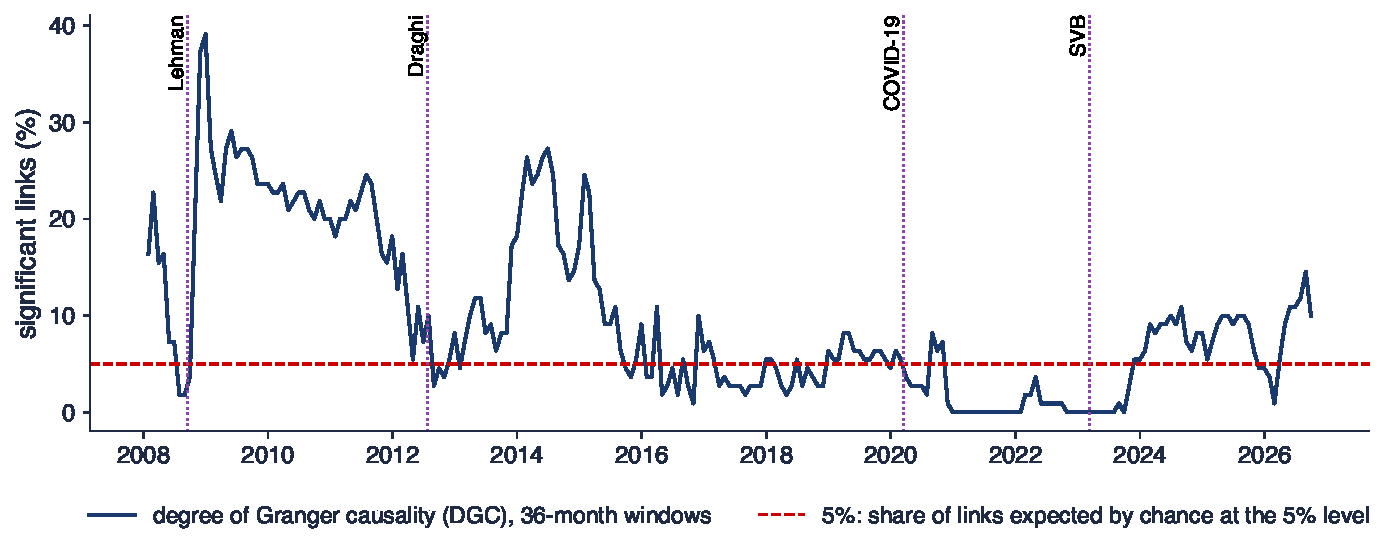
\includegraphics[width=0.97\textwidth,height=0.58\textheight,keepaspectratio]{sfm_ch15_dgc.pdf}
\end{center}
\vspace{-0.25cm}
\begin{itemize}
    \item 11 US and European banks, monthly returns since 2005 (260 months); first window ends in January 2008
    \item DGC: maximum 39\% (window ending 31 December 2008), average 10\%, minimum 0\% (31 December 2020)
\end{itemize}
\sfmquantlet{Ch_15}{SFM_ch15_networks}
\end{frame}

\begin{frame}{Two Networks: 2007--2009 and 2017--2019}
\itemsize{\footnotesize}
\begin{center}
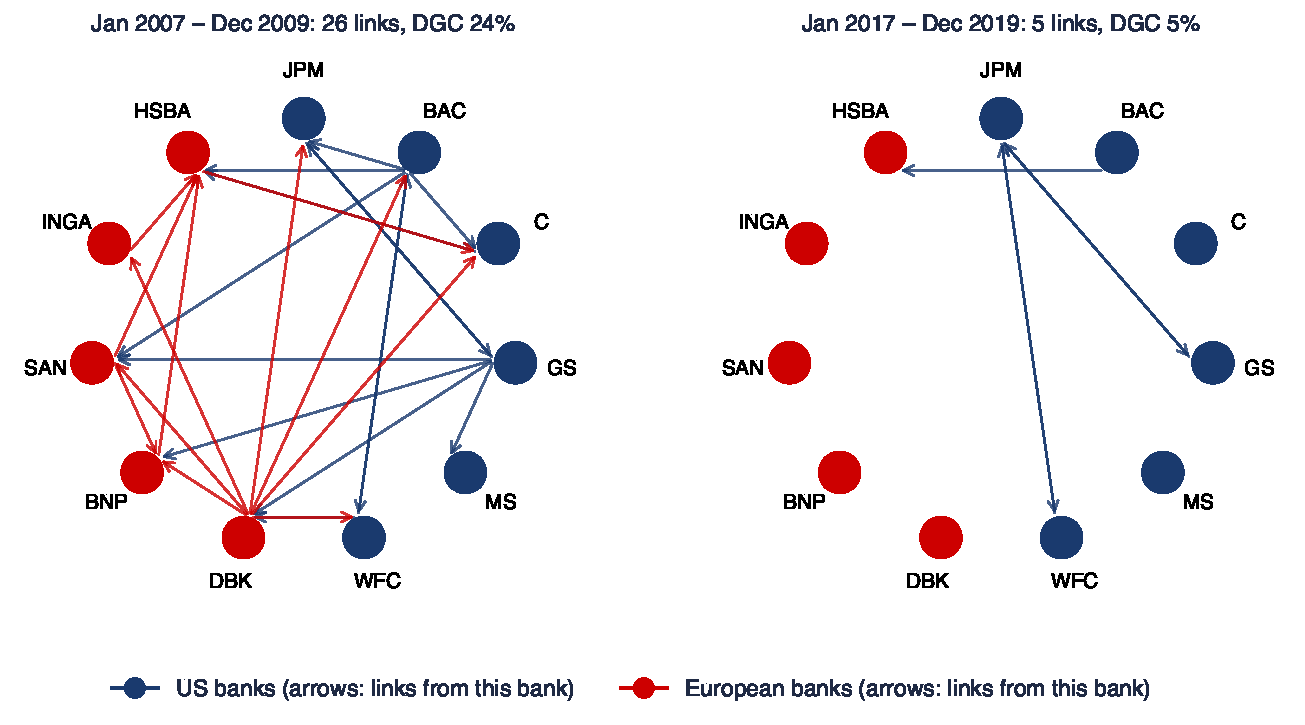
\includegraphics[width=0.97\textwidth,height=0.62\textheight,keepaspectratio]{sfm_ch15_granger_net.pdf}
\end{center}
\vspace{-0.25cm}
\begin{itemize}
    \item Arrows: significant Granger-causal links at 5\% in a 36-month window; 26 links in the crisis window, 5 in the calm one
    \item Interpretation: as in \refBGLP, the banks became more connected around the crisis; in calm years the network is close to what chance alone would give
\end{itemize}
\sfmquantlet{Ch_15}{SFM_ch15_networks}
\end{frame}

\begin{frame}{Diebold--Yilmaz Connectedness}
\itemsize{\small}
\begin{itemize}
    \item Fit a VAR (vector autoregression) to the returns of $N$ banks; forecast $H$ days ahead
    \begin{itemize}
        \item VAR($p$): $x_t = c + \Phi_1x_{t-1} + \dots + \Phi_px_{t-p} + u_t$; $x_t$: the vector of the $N$ returns; $\Phi_j$: $N \times N$ coefficient matrices; $u_t$: the shocks
        \item $d_{ij}$: the share of the $H$-day forecast error variance of bank $i$ due to shocks to bank $j$ (generalized decomposition, \refPS)
        \item each row sums to 100\%
    \end{itemize}
    \item Measures \refDYb; \refDYc
    \begin{itemize}
        \item FROM others: $\sum_{j \ne i} d_{ij}$; TO others: $\sum_{j \ne i} d_{ji}$; NET $=$ TO $-$ FROM
        \item \textbf{total connectedness}: $\frac{1}{N}\sum_{i \ne j} d_{ij}$, the average share of risk that comes from the others
    \end{itemize}
    \item Here: daily returns of 11 banks since 2005, VAR order by BIC (Bayesian information criterion), $H = 10$ days
\end{itemize}
\end{frame}

\begin{frame}{The Connectedness Table}
\itemsize{\footnotesize}
\begin{center}
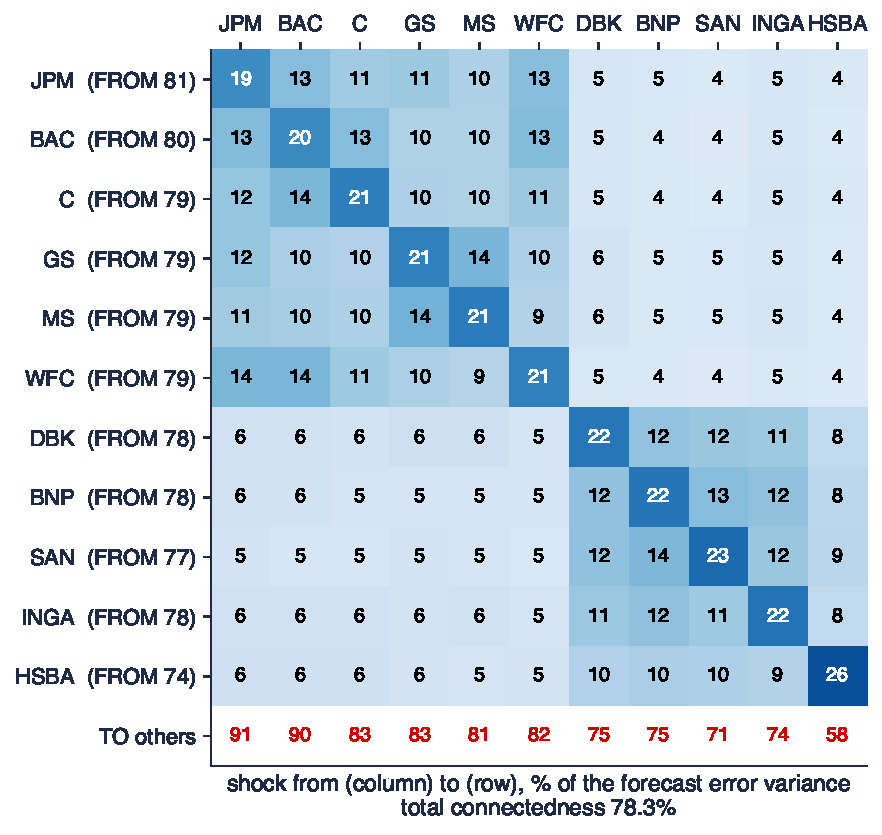
\includegraphics[width=0.97\textwidth,height=0.64\textheight,keepaspectratio]{sfm_ch15_dy_table.pdf}
\end{center}
\vspace{-0.25cm}
\begin{itemize}
    \item 4\,895 common days, VAR(1); total connectedness 78.3\%; two blocks: US banks are connected mostly with US banks, European with European
    \item Largest transmitter (TO): JPMorgan Chase; smallest: HSBC (NET $-15.8$)
\end{itemize}
\sfmquantlet{Ch_15}{SFM_ch15_networks}
\end{frame}

\begin{frame}{Interpretation of the Connectedness Table}
\itemsize{\small}
\begin{itemize}
    \item Each bank receives about four fifths of its forecast error variance from the others (FROM between 74 and 81)
    \begin{itemize}
        \item daily bank returns are dominated by common shocks; the own share (the diagonal) is only about one fifth
    \end{itemize}
    \item NET: US banks are net transmitters (JPMorgan Chase $+10.6$), European banks net receivers (HSBC $-15.8$)
    \begin{itemize}
        \item partly timing: New York closes after Europe, so US news reaches European prices the next day
    \end{itemize}
    \item Connectedness describes the data; it is not a map of exposures between the banks
\end{itemize}
\end{frame}

\begin{frame}{Total Connectedness through Time}
\itemsize{\footnotesize}
\begin{center}
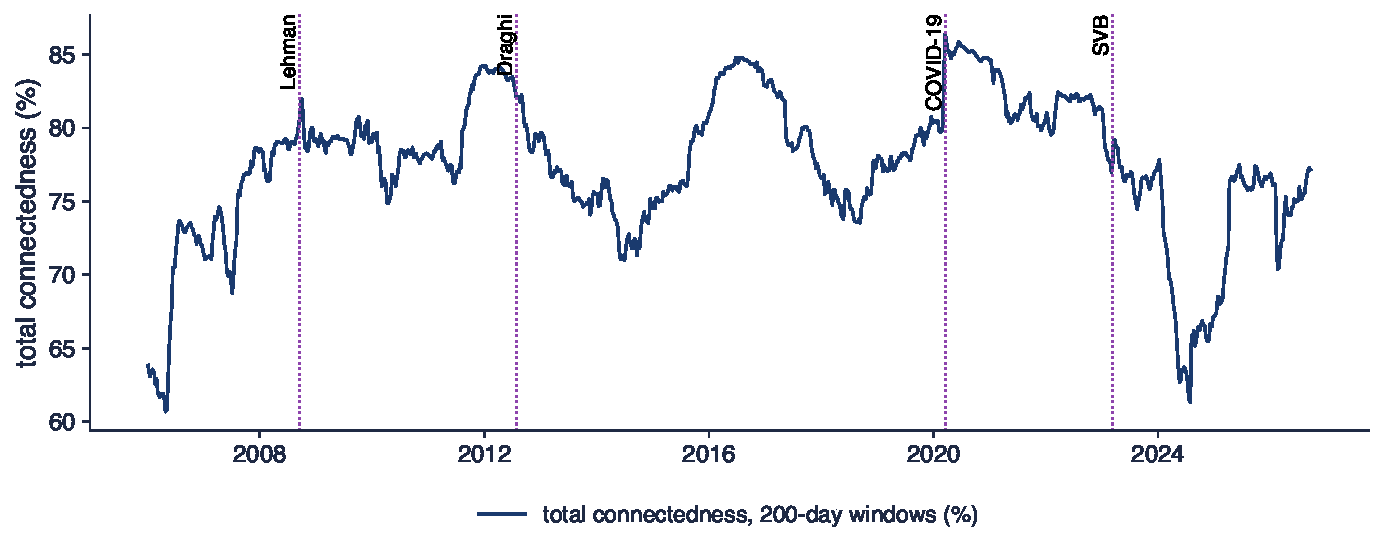
\includegraphics[width=0.97\textwidth,height=0.58\textheight,keepaspectratio]{sfm_ch15_dy_rolling.pdf}
\end{center}
\vspace{-0.25cm}
\begin{itemize}
    \item Rolling 200-day windows moved by 5 days; minimum 61\% (28 April 2006), maximum 86\% (17 March 2020); October 2008 -- March 2009: 79\%
    \item Interpretation: connectedness rose during 2007, before Lehman, and peaks in crises; it falls when bank-specific news dominate (2006, 2024)
\end{itemize}
\sfmquantlet{Ch_15}{SFM_ch15_networks}
\end{frame}

\begin{frame}{Further Reading: the Financial Risk Meter}
\itemsize{\small}
\begin{itemize}
    \item \textbf{FRM} (Financial Risk Meter) \refFRM: a daily index of systemic risk from quantile regressions with many regressors
    \begin{itemize}
        \item for each bank: a lasso quantile regression (\sfmchlink{https://danpele.github.io/SFM/EN/Courses/chapter13_machine_learning.pdf}{Chapter 13}) of its returns on the returns of all other banks and on macro variables
        \item the penalty $\lambda$ needed to fit the tail is large when the banks move together: FRM = the average $\lambda$
    \end{itemize}
    \item Extensions
    \begin{itemize}
        \item TENET (tail-event driven network) \refTENET: CoVaR with many banks, a network of tail links
        \item FRM for emerging markets \refFRMem; the video course on Quantinar (Reading and Tools)
    \end{itemize}
\end{itemize}
\end{frame}

\begin{frame}{Recap: Networks}
\itemsize{\small}
\begin{itemize}
    \item Granger networks: share of significant links (DGC) against the 5\% expected by chance; it rose around 2008
    \item Diebold--Yilmaz: shares of forecast error variance; TO, FROM, NET and the total index
    \item Statistical links show co-movement in the data; they do not reveal the contracts behind it
\end{itemize}
\end{frame}


%=============================================================================
\section{Macroprudential Policy}
%=============================================================================

\begin{frame}{Micro- and Macroprudential}
\itemsize{\small}
\begin{itemize}
    \item \textbf{Microprudential}: is each bank safe on its own? (capital, VaR, backtesting, \sfmchlink{https://danpele.github.io/SFM/EN/Courses/chapter10_var_es_backtesting.pdf}{Chapter 10})
    \item \textbf{Macroprudential}: is the system safe? Two dimensions
    \begin{itemize}
        \item \textbf{in time}: risk builds up in booms (credit growth, leverage) and shows in busts: build buffers in good times
        \item \textbf{across institutions}: larger and more connected banks need more capital
    \end{itemize}
    \item The measures of this chapter (CoVaR, SRISK, connectedness) are among the tools that central banks use to monitor the second dimension
\end{itemize}
\end{frame}

\begin{frame}{Basel III Capital Buffers}
\itemsize{\footnotesize}
\begin{columns}[T]
\begin{column}{0.62\textwidth}
\begin{itemize}
    \item Minimum CET1 (common equity tier 1) capital: 4.5\% of risk-weighted assets \refBIII; on top of it, buffers \refRBC:
    \begin{itemize}
        \item \textbf{capital conservation buffer}: 2.5\%; below it, dividends and bonuses are restricted
        \item \textbf{countercyclical buffer}: 0--2.5\%, raised when credit grows too fast, released in a crisis
    \end{itemize}
    \item For systemic importance
    \begin{itemize}
        \item \textbf{G-SIB surcharge}: 1\% to 3.5\%, by a score of size, interconnectedness, substitutability, complexity and cross-border activity \refGSIB
        \item in the EU: O-SII (other systemically important institutions) buffers and a systemic risk buffer
    \end{itemize}
\end{itemize}
\end{column}
\begin{column}{0.34\textwidth}
\centering
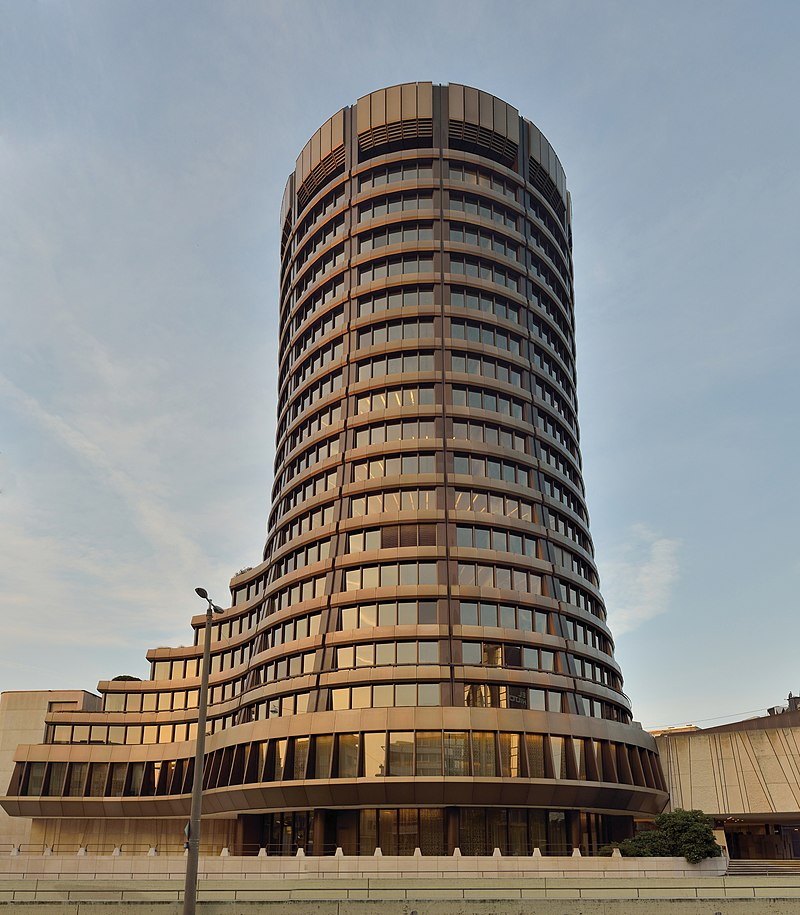
\includegraphics[height=0.36\textheight]{ch10_bis_tower_2014.jpg}\\[1mm]
\imgcap{The BIS tower in Basel}
\imgcredit{https://commons.wikimedia.org/wiki/File:Basel_Committee_on_Banking_Supervision_-_BCBS.jpg}{Photo: Taxiarchos228 (2014); CC BY-SA 4.0; Wikimedia Commons}
\end{column}
\end{columns}
\end{frame}

\begin{frame}{Who Does It: the ESRB and the BNR}
\itemsize{\footnotesize}
\begin{columns}[T]
\begin{column}{0.60\textwidth}
\begin{itemize}
    \item \textbf{ESRB} (European Systemic Risk Board), set up in 2010 after the crisis, chaired by the President of the ECB \refESRB
    \begin{itemize}
        \item monitors systemic risk in the EU, issues warnings and recommendations to national authorities
    \end{itemize}
    \item Romania: \textbf{CNSM} (Comitetul Național pentru Supravegherea Macroprudențială), with the BNR, the ASF (financial supervisory authority) and the Government \refCNSM
    \begin{itemize}
        \item the BNR sets the capital buffers of the banks (countercyclical, O-SII, systemic risk buffer) on CNSM recommendations
        \item the BNR also uses limits on borrowers (loan-to-value, debt service-to-income) and publishes a financial stability report
    \end{itemize}
\end{itemize}
\end{column}
\begin{column}{0.36\textwidth}
\centering
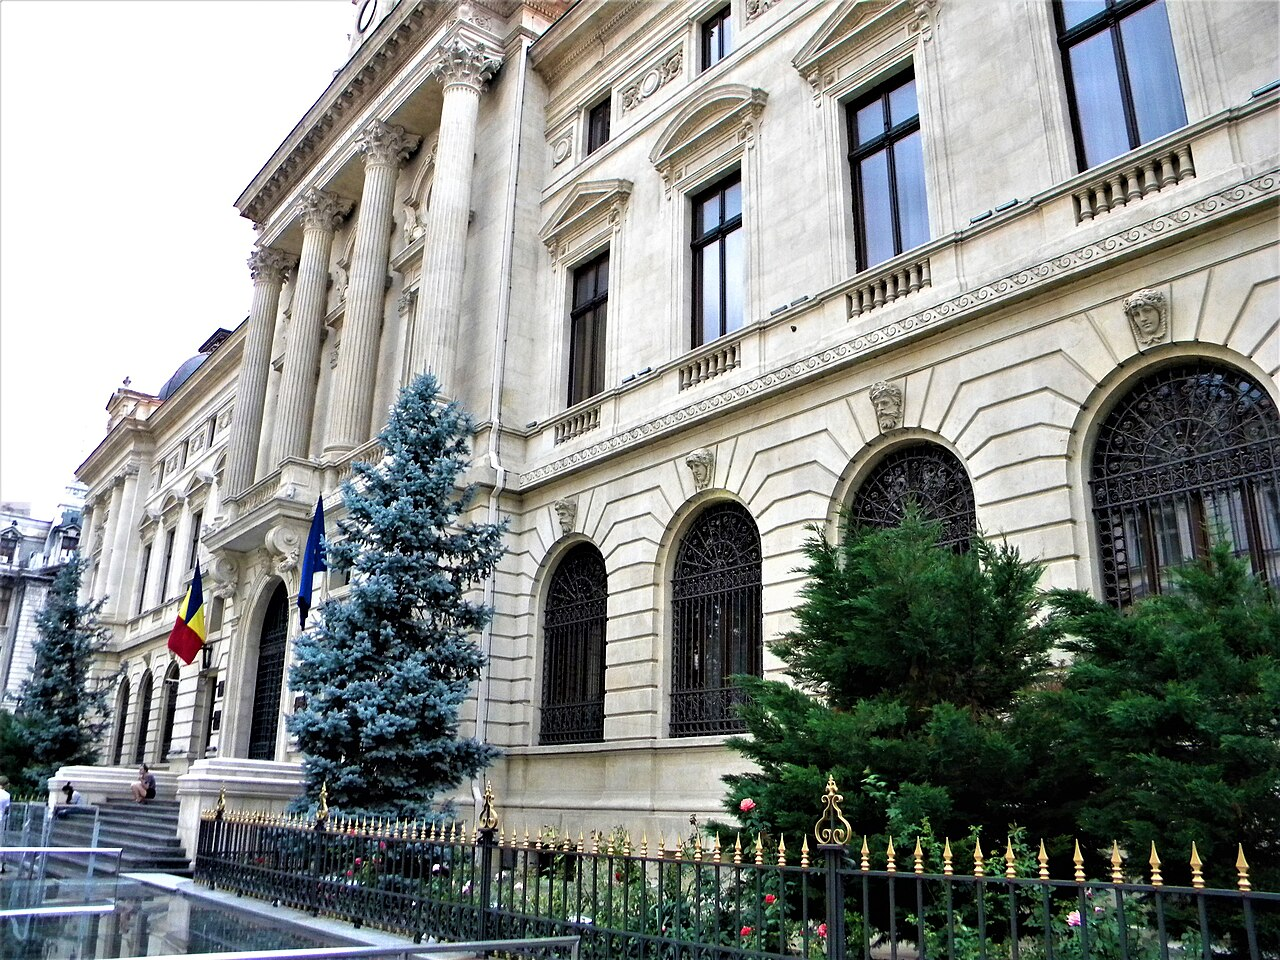
\includegraphics[height=0.36\textheight]{ch15_bnr_palace_2018.jpg}\\[1mm]
\imgcap{The BNR palace in Bucharest}
\imgcredit{https://commons.wikimedia.org/wiki/File:Bucuresti,_Romania._BANCA_NATIONALA_A_ROMANIEI_(2)_(B-II-m-A-19023).jpg}{Photo: Britchi Mirela (2018); CC BY-SA 4.0; Wikimedia Commons}
\end{column}
\end{columns}
\end{frame}

\begin{frame}{Recap: Macroprudential Policy}
\itemsize{\small}
\begin{itemize}
    \item Macroprudential policy targets the system: buffers built in good times, extra capital for systemic banks
    \item Basel III: 4.5\% CET1 + 2.5\% conservation + 0--2.5\% countercyclical + G-SIB / O-SII surcharges
    \item EU: the ESRB; Romania: the CNSM, with the BNR applying the capital buffers
\end{itemize}
\end{frame}


%=============================================================================
\section{AI for Scientific Discovery}
%=============================================================================

\begin{frame}{An Open Question}
\itemsize{\small}
\begin{itemize}
    \item \textbf{Is the systemic risk of the Romanian banks imported from their euro-area parents, or is it local?}
    \begin{itemize}
        \item today: $\Delta$CoVaR of TLV peaks in March 2020 ($12.81\%$); BRD belongs to a French group, TLV is Romanian-owned
        \item the BET is partly the banks themselves, so a better ``system'' is needed
    \end{itemize}
    \item Why it is open: two banks, few crises, different trading hours (Bucharest, Frankfurt, New York), thin trading in some years
    \item AI tools can speed up such a study; they do not replace checking it \refWang
\end{itemize}
\end{frame}

\begin{frame}{How AI Could Help}
\itemsize{\small}
\begin{itemize}
    \item \textbf{Literature}: a list of studies on systemic risk in Central and Eastern Europe and on parent--subsidiary contagion
    \item \textbf{Code}: a first draft of $\Delta$CoVaR of TLV and BRD with the euro-area bank portfolio as the conditioning variable and state variables
    \item \textbf{Robustness}: two-day returns (trading hours), weekly data, CoVaR at 5\%, other state variables
    \item Example prompt
    \begin{itemize}
        \item \aiprompt{Write Python code that estimates the Delta-CoVaR at 1\% of the BET conditional on Banca Transilvania by quantile regression, with the lagged VIX and the lagged Euro Stoxx 50 return as state variables, and adds a moving-block bootstrap interval.}
    \end{itemize}
\end{itemize}
\end{frame}

\begin{frame}{What to Check}
\itemsize{\small}
\begin{itemize}
    \item The level convention: ``CoVaR 1\%'' and ``MES 5\%'' name the tail probability; CoVaR and MES are positive losses
    \item The direction of conditioning: CoVaR is the system given the bank, MES is the bank given the market
    \item $\Delta$CoVaR compares distress with the \textbf{median} of the bank, not with the bank's VaR
    \item Prices joined on common days before returns; BVB days without trades removed; different trading hours
    \item Uncertainty: quantile regressions at 1\% rest on about 1\% of the days; report bootstrap intervals
    \item References: every cited paper must exist; check the DOI
\end{itemize}
\end{frame}

\begin{frame}{Project Idea}
\itemsize{\small}
\begin{itemize}
    \item \textbf{Question}: do the euro-area banks raise the tail risk of the Romanian banks in stress periods?
    \begin{itemize}
        \item data: TLV, BRD, BET, the five European banks, Euro Stoxx 50, VIX, since 2010 (EODHD)
    \end{itemize}
    \item Steps
    \begin{itemize}
        \item $\Delta$CoVaR 1\% of each Romanian bank conditional on the European bank portfolio, static and with state variables
        \item MES 5\% of TLV and BRD with the Euro Stoxx 50 as the market; Diebold--Yilmaz FROM shares on rolling windows
        \item compare 2011--2012, March 2020 and March 2023, with block-bootstrap intervals
    \end{itemize}
    \item Deliverable: one table, one chart, and a paragraph on what the data can and cannot show
    \item Declare any AI use, and list the errors of the AI that you corrected
\end{itemize}
\end{frame}


%=============================================================================
\section{Summary}
%=============================================================================

\begin{frame}{Key Takeaways}
\itemsize{\small}
\begin{itemize}
    \item Systemic risk is a property of the system: contagion, common exposures, fire sales and runs, amplified by leverage
    \item In crises bank correlations and tail dependence rise; correct for volatility before speaking of contagion
    \item CoVaR 1\%: the system given the bank; $\Delta$CoVaR $= \hat b(\hat q_{50\%} - \hat q_\alpha)$ from quantile regression
    \item MES 5\%: the bank given the market; SRISK $= kD - (1 - k)(1 - \mathrm{LRMES})W$, driven by leverage
    \item Networks (Granger, Diebold--Yilmaz) show more connectedness around crises
    \item Macroprudential policy: Basel III buffers, G-SIB and O-SII surcharges; the ESRB in the EU, the CNSM and the BNR in Romania
\end{itemize}
\end{frame}

\begin{frame}{Key Formulas}
\itemsize{\small}
{\renewcommand{\arraystretch}{1.45}\begin{center}
\scriptsize
\begin{tabular}{ll}
\toprule
\textbf{Quantity} & \textbf{Formula} \\
\midrule
CoVaR & $\mathrm{CoVaR}_\alpha = -(\hat a + \hat b\,\hat q_\alpha(X^i))$, \ $X^{sys} = a + bX^i$ at level $\alpha$ \\
$\Delta$CoVaR & $\hat b\,(\hat q_{50\%}(X^i) - \hat q_\alpha(X^i))$ \\
MES & $-E[X^i \mid X^m \le q_\alpha(X^m)]$ \\
LRMES & $1 - \exp(-18\,\mathrm{MES}_{2\%})$ \\
SRISK & $kD - (1 - k)(1 - \mathrm{LRMES})W$, \ $L^* = 1 + (1 - k)(1 - \mathrm{LRMES})/k$ \\
Forbes--Rigobon & $\rho^* = \rho/\sqrt{1 + \delta(1 - \rho^2)}$ \\
Granger & $y_t = a + by_{t-1} + cx_{t-1} + e_t$, \ $H_0: c = 0$ \\
Diebold--Yilmaz & total $= \frac1N\sum_{i \ne j} d_{ij}$, \ NET$_i = $ TO$_i - $ FROM$_i$ \\
\bottomrule
\end{tabular}
\end{center}
}
\end{frame}

\begin{frame}{Check Yourself}
\itemsize{\small}
\begin{itemize}
    \item \textbf{Question}: bank A has a larger VaR 1\% than bank B. Is A more systemic?
    \begin{itemize}
        \item \textbf{Answer}: not necessarily: systemic importance depends on the link with the system ($\Delta$CoVaR, MES), not on the bank's own tail
    \end{itemize}
    \item \textbf{Question}: a quantile regression at 1\% gives $\hat b = 0.5$, $\hat q_{1\%}(X^i) = -6\%$, $\hat q_{50\%}(X^i) = 0$. What is $\Delta$CoVaR?
    \begin{itemize}
        \item \textbf{Answer}: $0.5 \times (0 - (-6)) = 3\%$
    \end{itemize}
    \item \textbf{Question}: why can SRISK be negative?
    \begin{itemize}
        \item \textbf{Answer}: a bank with low leverage keeps enough capital even after a market fall of 40\%: it has a capital surplus
    \end{itemize}
    \item Next: \sfmchlink{https://danpele.github.io/SFM/EN/Courses/chapter16_review.pdf}{Chapter 16}, review
\end{itemize}
\end{frame}


%=============================================================================
\section{References}
%=============================================================================

\begin{frame}{References (1/3)}
\itemsize{\tiny}
\begin{itemize}
    \item Acharya, V.V., Engle, R., Richardson, M. (2012). \href{https://doi.org/10.1257/aer.102.3.59}{Capital shortfall: a new approach to ranking and regulating systemic risks}. \textit{American Economic Review}, 102(3), 59--64.
    \item Acharya, V.V., Pedersen, L.H., Philippon, T., Richardson, M. (2017). \href{https://doi.org/10.1093/rfs/hhw088}{Measuring systemic risk}. \textit{Review of Financial Studies}, 30(1), 2--47.
    \item Adrian, T., Brunnermeier, M.K. (2016). \href{https://doi.org/10.1257/aer.20120555}{CoVaR}. \textit{American Economic Review}, 106(7), 1705--1741.
    \item Allen, F., Gale, D. (2000). \href{https://doi.org/10.1086/262109}{Financial contagion}. \textit{Journal of Political Economy}, 108(1), 1--33.
    \item Basel Committee on Banking Supervision (2011). \href{https://www.bis.org/publ/bcbs189.htm}{Basel III: a global regulatory framework for more resilient banks and banking systems}, revised June 2011. Bank for International Settlements.
    \item Basel Committee on Banking Supervision (2018). \href{https://www.bis.org/bcbs/publ/d445.htm}{Global systemically important banks: revised assessment methodology and the higher loss absorbency requirement}. Bank for International Settlements.
    \item Ben Amor, S., Althof, M., Härdle, W.K. (2022). \href{https://doi.org/10.1016/j.ribaf.2021.101594}{Financial Risk Meter for emerging markets}. \textit{Research in International Business and Finance}, 60, 101594.
    \item Benoit, S., Colliard, J.-E., Hurlin, C., Pérignon, C. (2017). \href{https://doi.org/10.1093/rof/rfw026}{Where the risks lie: a survey on systemic risk}. \textit{Review of Finance}, 21(1), 109--152.
    \item Billio, M., Getmansky, M., Lo, A.W., Pelizzon, L. (2012). \href{https://doi.org/10.1016/j.jfineco.2011.12.010}{Econometric measures of connectedness and systemic risk in the finance and insurance sectors}. \textit{Journal of Financial Economics}, 104(3), 535--559.
    \item Bisias, D., Flood, M., Lo, A.W., Valavanis, S. (2012). \href{https://doi.org/10.1146/annurev-financial-110311-101754}{A survey of systemic risk analytics}. \textit{Annual Review of Financial Economics}, 4, 255--296.
    \item Brownlees, C., Engle, R.F. (2017). \href{https://doi.org/10.1093/rfs/hhw060}{SRISK: a conditional capital shortfall measure of systemic risk}. \textit{Review of Financial Studies}, 30(1), 48--79.
    \item Brunnermeier, M.K., Pedersen, L.H. (2009). \href{https://doi.org/10.1093/rfs/hhn098}{Market liquidity and funding liquidity}. \textit{Review of Financial Studies}, 22(6), 2201--2238.
    \item Demarta, S., McNeil, A.J. (2005). \href{https://doi.org/10.1111/j.1751-5823.2005.tb00254.x}{The t copula and related copulas}. \textit{International Statistical Review}, 73(1), 111--129.
    \item Diamond, D.W., Dybvig, P.H. (1983). \href{https://doi.org/10.1086/261155}{Bank runs, deposit insurance, and liquidity}. \textit{Journal of Political Economy}, 91(3), 401--419.
    \item Diebold, F.X., Yilmaz, K. (2009). \href{https://doi.org/10.1111/j.1468-0297.2008.02208.x}{Measuring financial asset return and volatility spillovers, with application to global equity markets}. \textit{Economic Journal}, 119(534), 158--171.
    \item Diebold, F.X., Yilmaz, K. (2012). \href{https://doi.org/10.1016/j.ijforecast.2011.02.006}{Better to give than to receive: predictive directional measurement of volatility spillovers}. \textit{International Journal of Forecasting}, 28(1), 57--66.
\end{itemize}
\end{frame}

\begin{frame}{References (2/3)}
\itemsize{\tiny}
\begin{itemize}
    \item Diebold, F.X., Yilmaz, K. (2014). \href{https://doi.org/10.1016/j.jeconom.2014.04.012}{On the network topology of variance decompositions: measuring the connectedness of financial firms}. \textit{Journal of Econometrics}, 182(1), 119--134.
    \item Draghi, M. (2012). \href{https://www.ecb.europa.eu/press/key/date/2012/html/sp120726.en.html}{Speech at the Global Investment Conference}, London, 26 July 2012. European Central Bank.
    \item Engle, R., Jondeau, E., Rockinger, M. (2015). \href{https://doi.org/10.1093/rof/rfu012}{Systemic risk in Europe}. \textit{Review of Finance}, 19(1), 145--190.
    \item European Systemic Risk Board (2026). \href{https://www.esrb.europa.eu/about/background/html/index.en.html}{Background and tasks}. Frankfurt am Main.
    \item Federal Deposit Insurance Corporation (2023). \href{https://www.fdic.gov/resources/resolutions/bank-failures/failed-bank-list/silicon-valley.html}{Silicon Valley Bank, Santa Clara, CA}. Failed bank information.
    \item Federal Reserve Board (2023). \href{https://www.federalreserve.gov/publications/files/svb-review-20230428.pdf}{Review of the Federal Reserve's supervision and regulation of Silicon Valley Bank}. Washington, DC, April 2023.
    \item FINMA (2023). \href{https://www.finma.ch/en/news/2023/03/20230319-mm-cs-ubs/}{FINMA approves merger of Credit Suisse and UBS}. Press release, 19 March 2023.
    \item Forbes, K.J., Rigobon, R. (2002). \href{https://doi.org/10.1111/0022-1082.00494}{No contagion, only interdependence: measuring stock market comovements}. \textit{Journal of Finance}, 57(5), 2223--2261.
    \item Franke, J., Härdle, W.K., Hafner, C.M. (2019). \href{https://doi.org/10.1007/978-3-030-13751-9}{\textit{Statistics of Financial Markets: An Introduction}}, 5th ed. Springer.
    \item Granger, C.W.J. (1969). \href{https://doi.org/10.2307/1912791}{Investigating causal relations by econometric models and cross-spectral methods}. \textit{Econometrica}, 37(3), 424--438.
    \item Haldane, A.G., May, R.M. (2011). \href{https://doi.org/10.1038/nature09659}{Systemic risk in banking ecosystems}. \textit{Nature}, 469, 351--355.
    \item Härdle, W.K., Wang, W., Yu, L. (2016). \href{https://doi.org/10.1016/j.jeconom.2016.02.013}{TENET: Tail-Event driven NETwork risk}. \textit{Journal of Econometrics}, 192(2), 499--513.
    \item IMF, BIS, FSB (2009). \href{https://www.bis.org/publ/othp07.htm}{Guidance to assess the systemic importance of financial institutions, markets and instruments: initial considerations}. Report to the G-20 Finance Ministers and Central Bank Governors.
    \item Koenker, R., Bassett, G. (1978). \href{https://doi.org/10.2307/1913643}{Regression quantiles}. \textit{Econometrica}, 46(1), 33--50.
    \item Mihoci, A., Althof, M., Chen, C.Y.-H., Härdle, W.K. (2020). \href{https://doi.org/10.1108/s0731-905320200000042016}{FRM Financial Risk Meter}. In \textit{The Econometrics of Networks}, Advances in Econometrics, 42, 335--368. Emerald.
    \item National Committee for Macroprudential Oversight (CNSM) (2026). \href{https://www.cnsmro.ro/}{Comitetul Național pentru Supravegherea Macroprudențială}. Bucharest.
\end{itemize}
\end{frame}

\begin{frame}{References (3/3)}
\itemsize{\tiny}
\begin{itemize}
    \item Pesaran, H.H., Shin, Y. (1998). \href{https://doi.org/10.1016/S0165-1765(97)00214-0}{Generalized impulse response analysis in linear multivariate models}. \textit{Economics Letters}, 58(1), 17--29.
    \item Shleifer, A., Vishny, R. (2011). \href{https://doi.org/10.1257/jep.25.1.29}{Fire sales in finance and macroeconomics}. \textit{Journal of Economic Perspectives}, 25(1), 29--48.
    \item Wang, H., Fu, T., Du, Y., Gao, W., et al. (2023). \href{https://doi.org/10.1038/s41586-023-06221-2}{Scientific discovery in the age of artificial intelligence}. \textit{Nature}, 620, 47--60.
\end{itemize}
\end{frame}

\end{document}
